\chapter{Infinity and recursion}

The \isi{object metaphor} makes it possible to view human language as the output of a recursive procedure. This recursive procedure, \textsc{Merge}, the essence of the human language faculty (\citeauthor{Chomsky2001b} \citeyear*{Chomsky2001b,Chomsky2008}), yields an \isi{infinite set} of sentences -- or so it is said. An early expression of this view, according to \citet{Tomalin2007}, appears in \citet{Bar-Hillel1953recursive}, who observed that recursive definitions could be useful in linguistics. The linguistic use of connected object structures, which provide a conceptual basis for \isi{recursion}, originates even earlier, tracing back to the German psychologist Wilhelm Wundt (1832--1920) \citep{Seuren1998}.

  But if one chooses not to view language as structures of connected objects, the notion of a capacity for discrete \isi{infinity} becomes absurd. In this chapter we examine how the \isi{object metaphor} is used to construct recursive \textsc{Merge}, and develop an alternative way of thinking about \isi{recursion} in the o/el paradigm. There is a superficial critique of the notion that \isi{recursion} is the essence of the human language faculty, based on evidence that there may be languages without “\isi{recursion}” \citep{Everett2005}. That particular critique is counterproductive in my view, because it presupposes the conventional framework. The deeper critique is that thinking of language as “recursive” is only possible when presupposing the \isi{object metaphor}. When we adopt an o/el conception, there are no capacities for \isi{infinity} that need explanation; \isi{recursion} is merely an artifact of a particular conceptual model.

\section{The infinite set conception of language}

The “infinite” nature of language has been a key argument against a finite-state model in favor of a \isi{phrase structure} grammar. The logic of the argument is that languages are infinite sets of sentences, which can include dependencies that are infinite, and a finite-state model cannot produce sentences with infinite dependencies. (Note that a finite-state model \textit{can} produce infinitely long sentences with finite dependencies). One problem with the logic of this argument is the tenet that languages \textit{are} sets of sentences. Let's examine some of what has been written about this idea.  

By a language, then, we shall mean a set (finite or infinite) of sentences, each of finite length, all constructed from a finite alphabet of symbols \citep[114]{Chomsky1956}.

\begin{quote}
    There are infinite sets of sentences that have dependency sets with more than any fixed number of terms \citep[115]{Chomsky1956}. 
    \end{quote}

The construct of the \isi{infinite set} has been extended to thoughts as well:

\begin{quote}
The ability to embed a proposition inside another proposition bestows the ability to think an infinite number of thoughts \citep[125]{Pinker1999}. 
\end{quote}

  Where does the \isi{infinite set conception} of language come from? Chomsky himself identified it as an assumption, arguing that if languages were finite sets of sentences generated by a non-recursive grammar (e.g. a finite state model), then that grammar would have to be very complicated:
  
\begin{quote}
In general, the assumption that languages are infinite is made for the purpose of simplifying the description. If a grammar has no recursive steps\ldots it will be prohibitively complex -- it will, in fact, turn out to be little better than a list of strings or of morpheme class sequences in the case of natural languages. If it does have recursive devices, it will produce infinitely many sentences (1956: 115--116).
\end{quote}

  The reasoning is that if grammars were non-recursive, we would have a tough time describing them. There is a circularity in this reasoning: “prohibitive” complexity of a description is only \textit{prohibitive} in a certain (object-based) construal of what the description could be. As sensible as this reasoning seems within the conventional paradigm, it is not -- from a theory-external perspective -- a satisfying argument for the \isi{infinite set conception}. Indeed, from a more neutral perspective, the prohibitive complexity of describing sentences in a finite way might be taken as an argument that language should \textit{not} be conceptualized as structures of objects/symbols in the first place.

  There are two aspects of the \isi{infinite set conception} that we call into question here: 
  (1) whether it is sensible to think of the set of sentences \textit{as infinite}, and 
  (2) whether it is sensible to think of language \textit{as a set of sentences}. To aid these critiques we employ an object collection schema (cf. \citealt{LakoffNúñez2000}) with pebbles as objects. The schema is as follows: 

\begin{quote}
    Picture an infinite beach of pebbles, of various sizes and compositions. We take one pebble at a time and add it to our infinitely large bag. If we imagine doing this forever, we obtain an \isi{infinite set} of pebbles. 
\end{quote}

  There are many ways in which the infinite pebble collection is analogous to the \isi{infinite set} of sentences in conventional approaches. First, all of the sentences we add to our collection will be \textit{different} in the sense that no two sentences in our set have identical “structure”, but they are all the \textit{same type} of thing, i.e. a “sentence”, which we may feel obligated to define. The same holds for the pebble collection: no two pebbles in our set of pebbles have \textit{identical} structure, but they are all the \textit{same type} of thing, i.e. a “pebble”. 
  
  We should also feel obligated to define what a pebble is. Both pebbles and sentences are categories that we construct. There is no objective, physically defined, model-independent notion of a sentence, nor is there an objective category of a pebble. On a relatively macroscopic scale, all pebbles are solid objects composed of various crystalline grains, but on a smaller scale, we can only describe pebbles as spatial organizations of molecules, and on an even smaller scale, as quantum wavefunctions. To count pebbles as “pebbles”, we must construct a sufficiently general category, \textsc{pebble}, by making reference to relatively microscopic constructs such as molecules. Yet one can always contest the category, on the basis of its scale-dependence. The same holds for sentences: on a relatively macroscopic scale, the \isi{object metaphor} allows us to view sentences as unique spatial arrangements of linguistic units, but on a smaller scale, we must describe them as very high-di\-men\-sional spatiotemporal patterns of neural activity. On that view, no two utterances of \textit{Al drinks coffee} are identical. Thus the categories of \textsc{sentence} and \textsc{pebble} are analytical impositions -- constructs, associated with a macroscopic analysis. 

  In the analogy, the bag of pebbles is a language, i.e. a set of sentences -- the bag is the set. This works well because sets are container schemas. The mathematical notion of a classical set is, via its fundamental metaphor, based on a \isi{container schema} \citep{LakoffNúñez2000}. This makes it sensible to refer to numbers as being “inside” or “outside” of sets, but not partly inside, and never both inside and outside. Likewise, a sentence is either in a language or not, just as a pebble is either in the bag or not. The sentences and pebbles are objects, and we can imagine an infinitely long sentence, and an infinitely large pebble -- both are objects. 

  The processes of collecting an infinite number of pebbles and generating an \isi{infinite set} of sentences have an important similarity: we imagine them iteratively, and occurring forever. Our conception of \isi{infinity} is not, in its most basic form, an \isi{atemporal} concept. We do not convince ourselves of the possibility of \isi{infinity} with the snap of a finger. Instead, we believe in infinities because we can imagine iterating actions, like dropping pebbles into a bag or adding sentences to a set. This observation suggests that we should think more carefully about \isi{infinity} as a human construct, distinguishing as Aristotle did between an imagined potential for \isi{infinity} and \isi{infinity} in actuality (see \citealt{Lear1988}).

\subsection{Potential infinity is not very special}

There are some mathematicians, \textit{finitists}, who accept the existence of only finite mathematical objects. Historically, \isi{infinity} is an old idea, but it \textit{is} just an idea, and hence it is contestable. Carl Friedrich Gauss, Henri Poincaré, and Ludwig Wittgenstein all questioned the existence of infinities: 

\begin{quote}
Gauss: I protest against the use of infinite magnitude as something completed, which is never permissible in mathematics. The Infinite is just a manner of speaking, in which one is really talking in terms of limits, which certain ratios may approach as close as one wishes, while others may be allowed to increase without restriction. (see \citealt{Waterhouse1979})
\end{quote}

\begin{quote}
Poincaré: There is no actual \isi{infinity}, that the Cantorians have forgotten, and have been trapped by contradictions. It is true that Cantorism rendered services, but that was when it was applied to a real problem whose terms were clearly defined, and we could walk safely. Logisticians as Cantorians have forgotten. (see \citealt{PoincaréMaitland2003}) 
\end{quote}

\begin{quote}
Wittgenstein: Let's imagine a man whose life goes back for an infinite time and who says to us: “I'm just writing down the last digit to Pi and it's 2”. Every day of his life he has written down a digit, without ever having begun; he has just finished. This seems utter nonsense, and a reductio ad absurdum of the concept of infinite totality. (see \citealt{Wittgenstein1980}).
\end{quote}

  The \textit{ideation} of \isi{infinity} comes from the same conceptual operation which constructs the integers: adding. In the object collection schema, take a pebble, add it to your bag, and repeat. Or in a path schema, take a step, add one, repeat. It does not matter that in actuality we would eventually run out of pebbles, or energy to take steps, because we can \textit{imagine} iterating these processes forever. There is nothing particularly special about the idea of constructing an \isi{infinite set}, i.e. a potential \isi{infinity}. Whether the set may be of sentences, or pebbles, or steps, or whatever. We can imagine that \textit{any} type of object can be constructed so that each member of the category is unique, and we can imagine doing this indefinitely. The point is that if one maintains that language is a capacity to produce an \isi{infinite set} of sentences, this can only mean that one imposes the necessary metaphors and schemas that allow a conceptual mapping between the act of collecting sentences and an imagined iteration of collecting objects. Whether there is anything particularly special or interesting about the imposition is a different issue.

\subsection{Language is not a set}

The other problem with the \isi{infinite set conception} is the notion of language \textit{as a set of sentences}. Is it sensible to think of a language as a \textit{set}? The Poincaré comment above is relevant here: \isi{infinity} is a useful tool when applied to a problem \textit{whose terms are clearly defined}. In order to view languages as sets of sentences, a “sentence” should be a clearly defined thing. Is this really the case? The typical maneuver is to assume a definition:

\begin{quote}
We may assume for this discussion that certain sequences of phonemes are definitely sentences, and that certain other sequences of phonemes are definitely non-sentences \citep[14]{Chomsky1957}.
\end{quote}

  But even when more serious definitional attempts are made, all such attempts suffer from a deeper problem: not all “parts” of sentence-objects are necessarily the same sort of thing. This means that thinking of sentences as “objects” which are collectable is misguided. Consider the object-collection schema for an \isi{infinite set}. Each new object (e.g. pebble, sentence) added to the collection is assumed to be “the same” as the previous objects. For another simple example, consider the set construction of the natural numbers. Each “1” that is added to the previous natural number to get the next natural number is the same as the previous “1”. It would be quite strange if that were not the case. Imagine if at some point we added the quasi-number 1* instead of 1:

  \ea
    1 + 1 = 2, \quad 2 + 1 = 3, \quad 3 + 1 = 4, \quad 4 + 1* = ?
\z

  What does it mean to add 1*? It is simply not defined, until we define it. Why label it 1*? Well, it is different from the 1s that we added previously. 1* is not the same sort of thing as 1, and so we cannot add it to anything in the set. This same point applies to language. Consider a classic example, \isi{tail recursion}:
\ea
\ea
{Al knows Bo drinks coffee.}
\ex
{Al knows Bo knows Cam drinks coffee.}
\ex
{Al knows Bo knows Cam knows Dee drinks coffee.}
\ex
{Al knows Bo knows Cam knows Dee knows Ed drinks coffee.}
\ex
{Al knows Bo knows Cam knows Dee knows Ed knows Fay knows…}
\z
\z

In the conventional view each of the sentences above is a structure of objects, all of which are \textit{simultaneously there}, in an occupiable space, i.e. \textit{co-present}. This is the implication of connected object structures such as in {\figref{fig:5:1}}(A). But in the o/el framework a configuration such as {\figref{fig:5:1}}(B) is unstable because of \isi{interference}; all of the cs-sys\-tems in (B) cannot be simultaneously excited. 

  
\begin{figure}
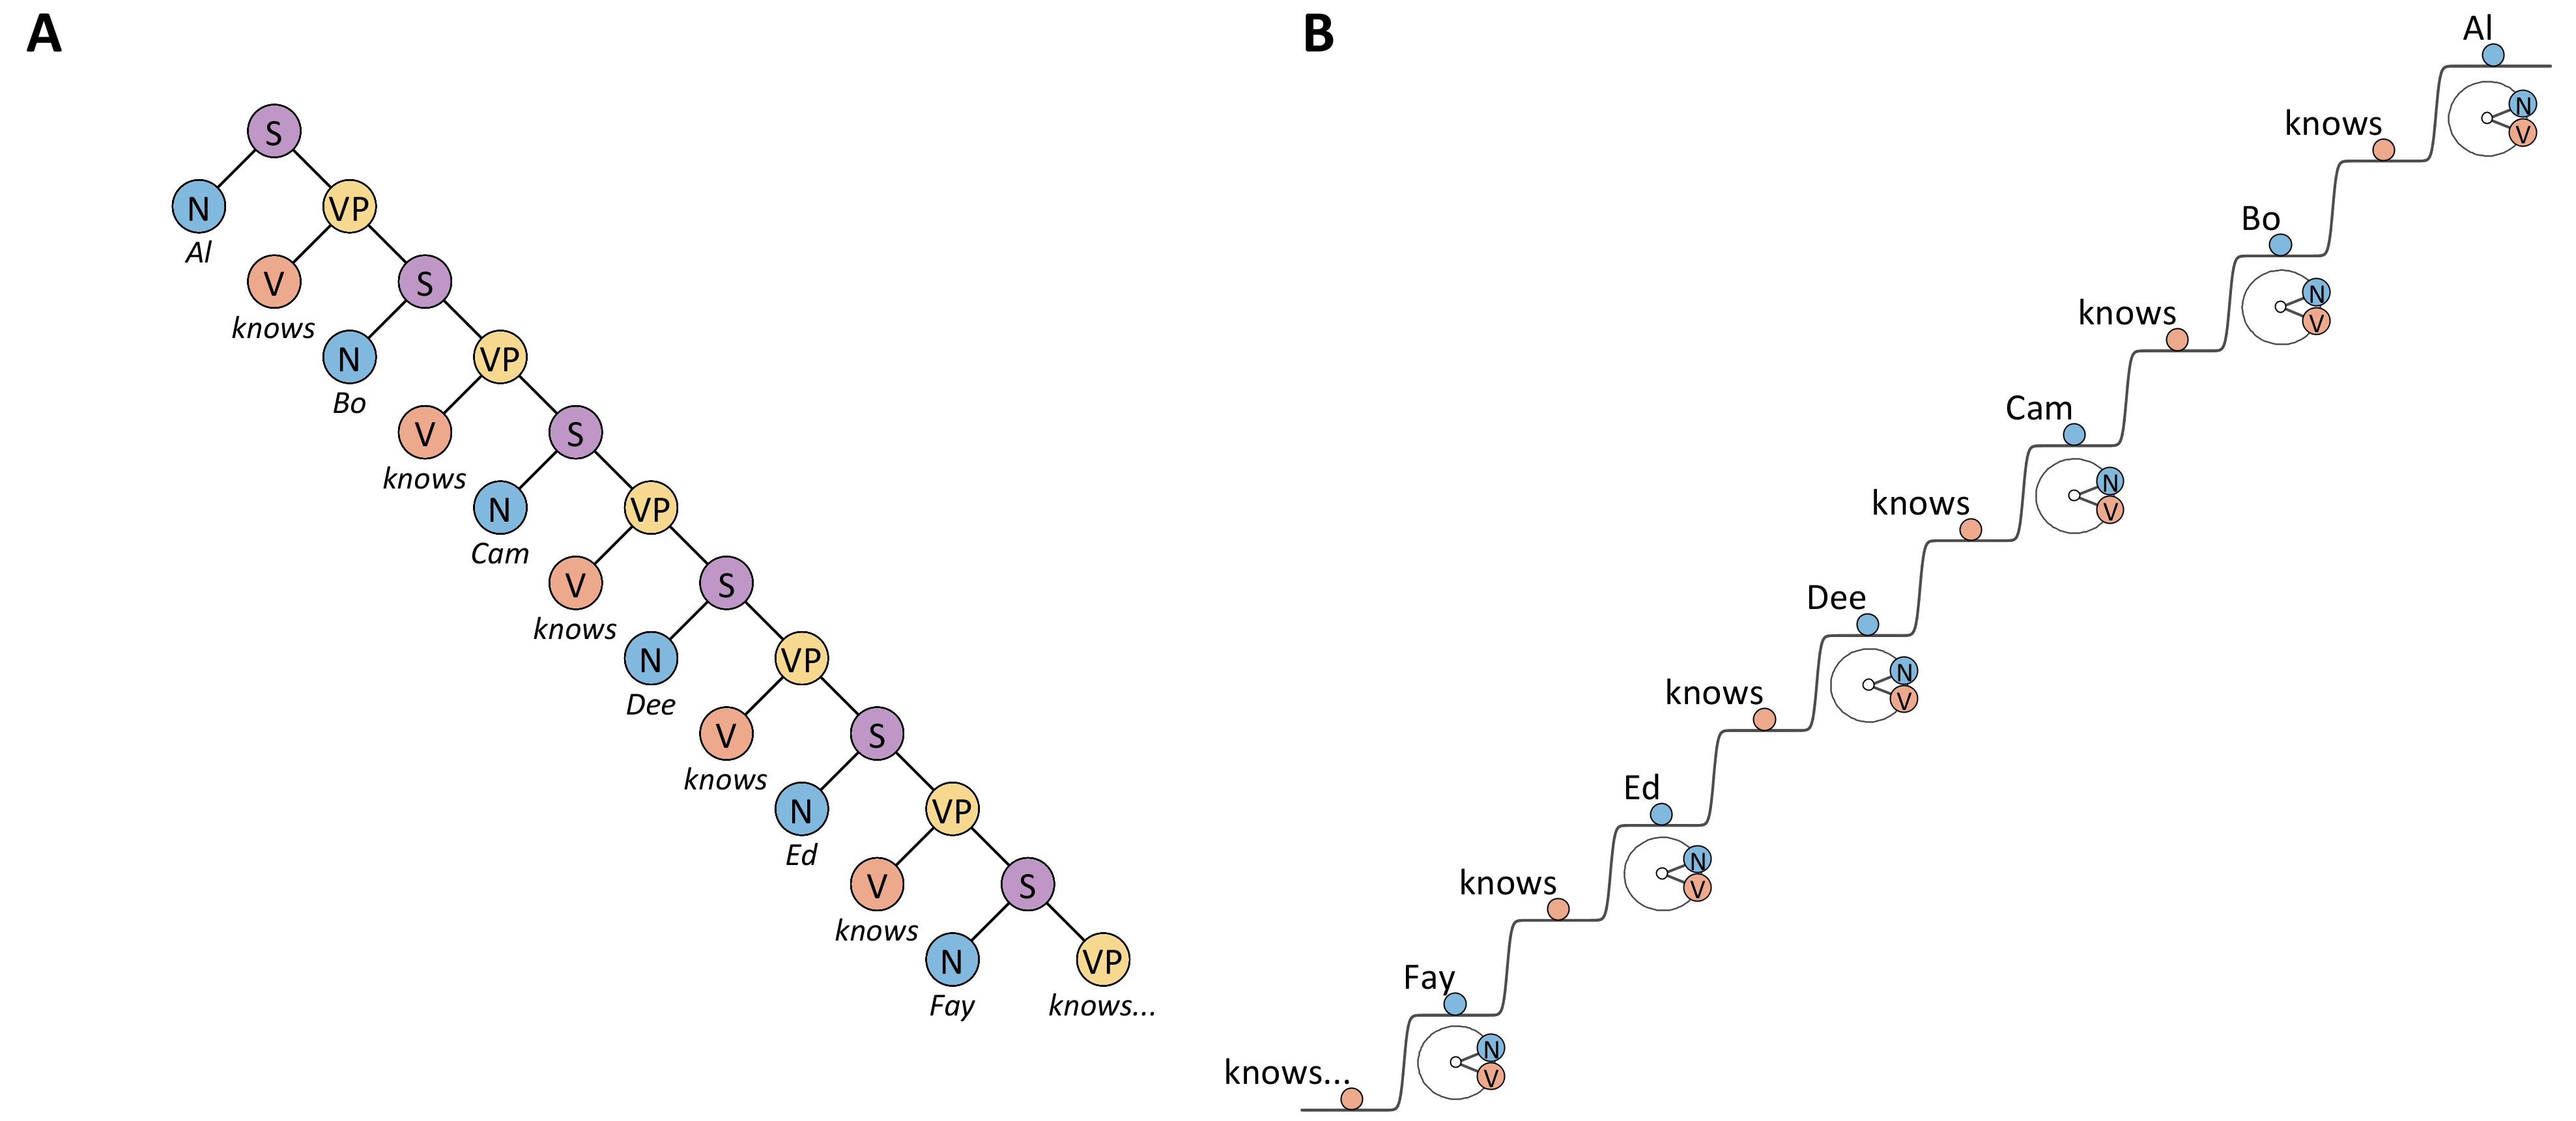
\includegraphics[width=\textwidth]{figures/Tilsen-img105.png}
\caption{Simultaneous presence of syntactic objects.}
\label{fig:5:1}
\end{figure}
 

  Instead of imposing simultaneity, the o/el framework imagines a sequence of epochs (e\textsubscript{1}…e\textsubscript{n}) as in {\figref{fig:5:2}}. Only a small set of relational meanings is attended in each epoch. For example, in (e1) the {\textbar}Al knows{\textbar} configuration is excited, while other systems are active. {\textbar}Al knows{\textbar} remains attended through the \isi{canonical reorganization} to (e2),  but a \isi{selective reorganization} occurs in the transition to (e3), such that {\textbar}Bo knows{\textbar} becomes excited and {\textbar}Al knows{\textbar} is demoted to ground. The pattern of \isi{canonical reorganization} and \isi{selective reorganization} can be iterated indefinitely, but there is nothing particularly special about a state that evolves in time. Crucially, the system is typically \textit{not} in a state where \isi{relational meaning} configurations associated with more than one (or perhaps a couple) clauses are highly excited. Hence \textit{Al knows Bo knows Cam knows…} is not one countable event, but rather, a succession of states. All of the clauses are never co-present in this view, and therefore \textit{they are not the same sort of thing}.

  
\begin{figure}
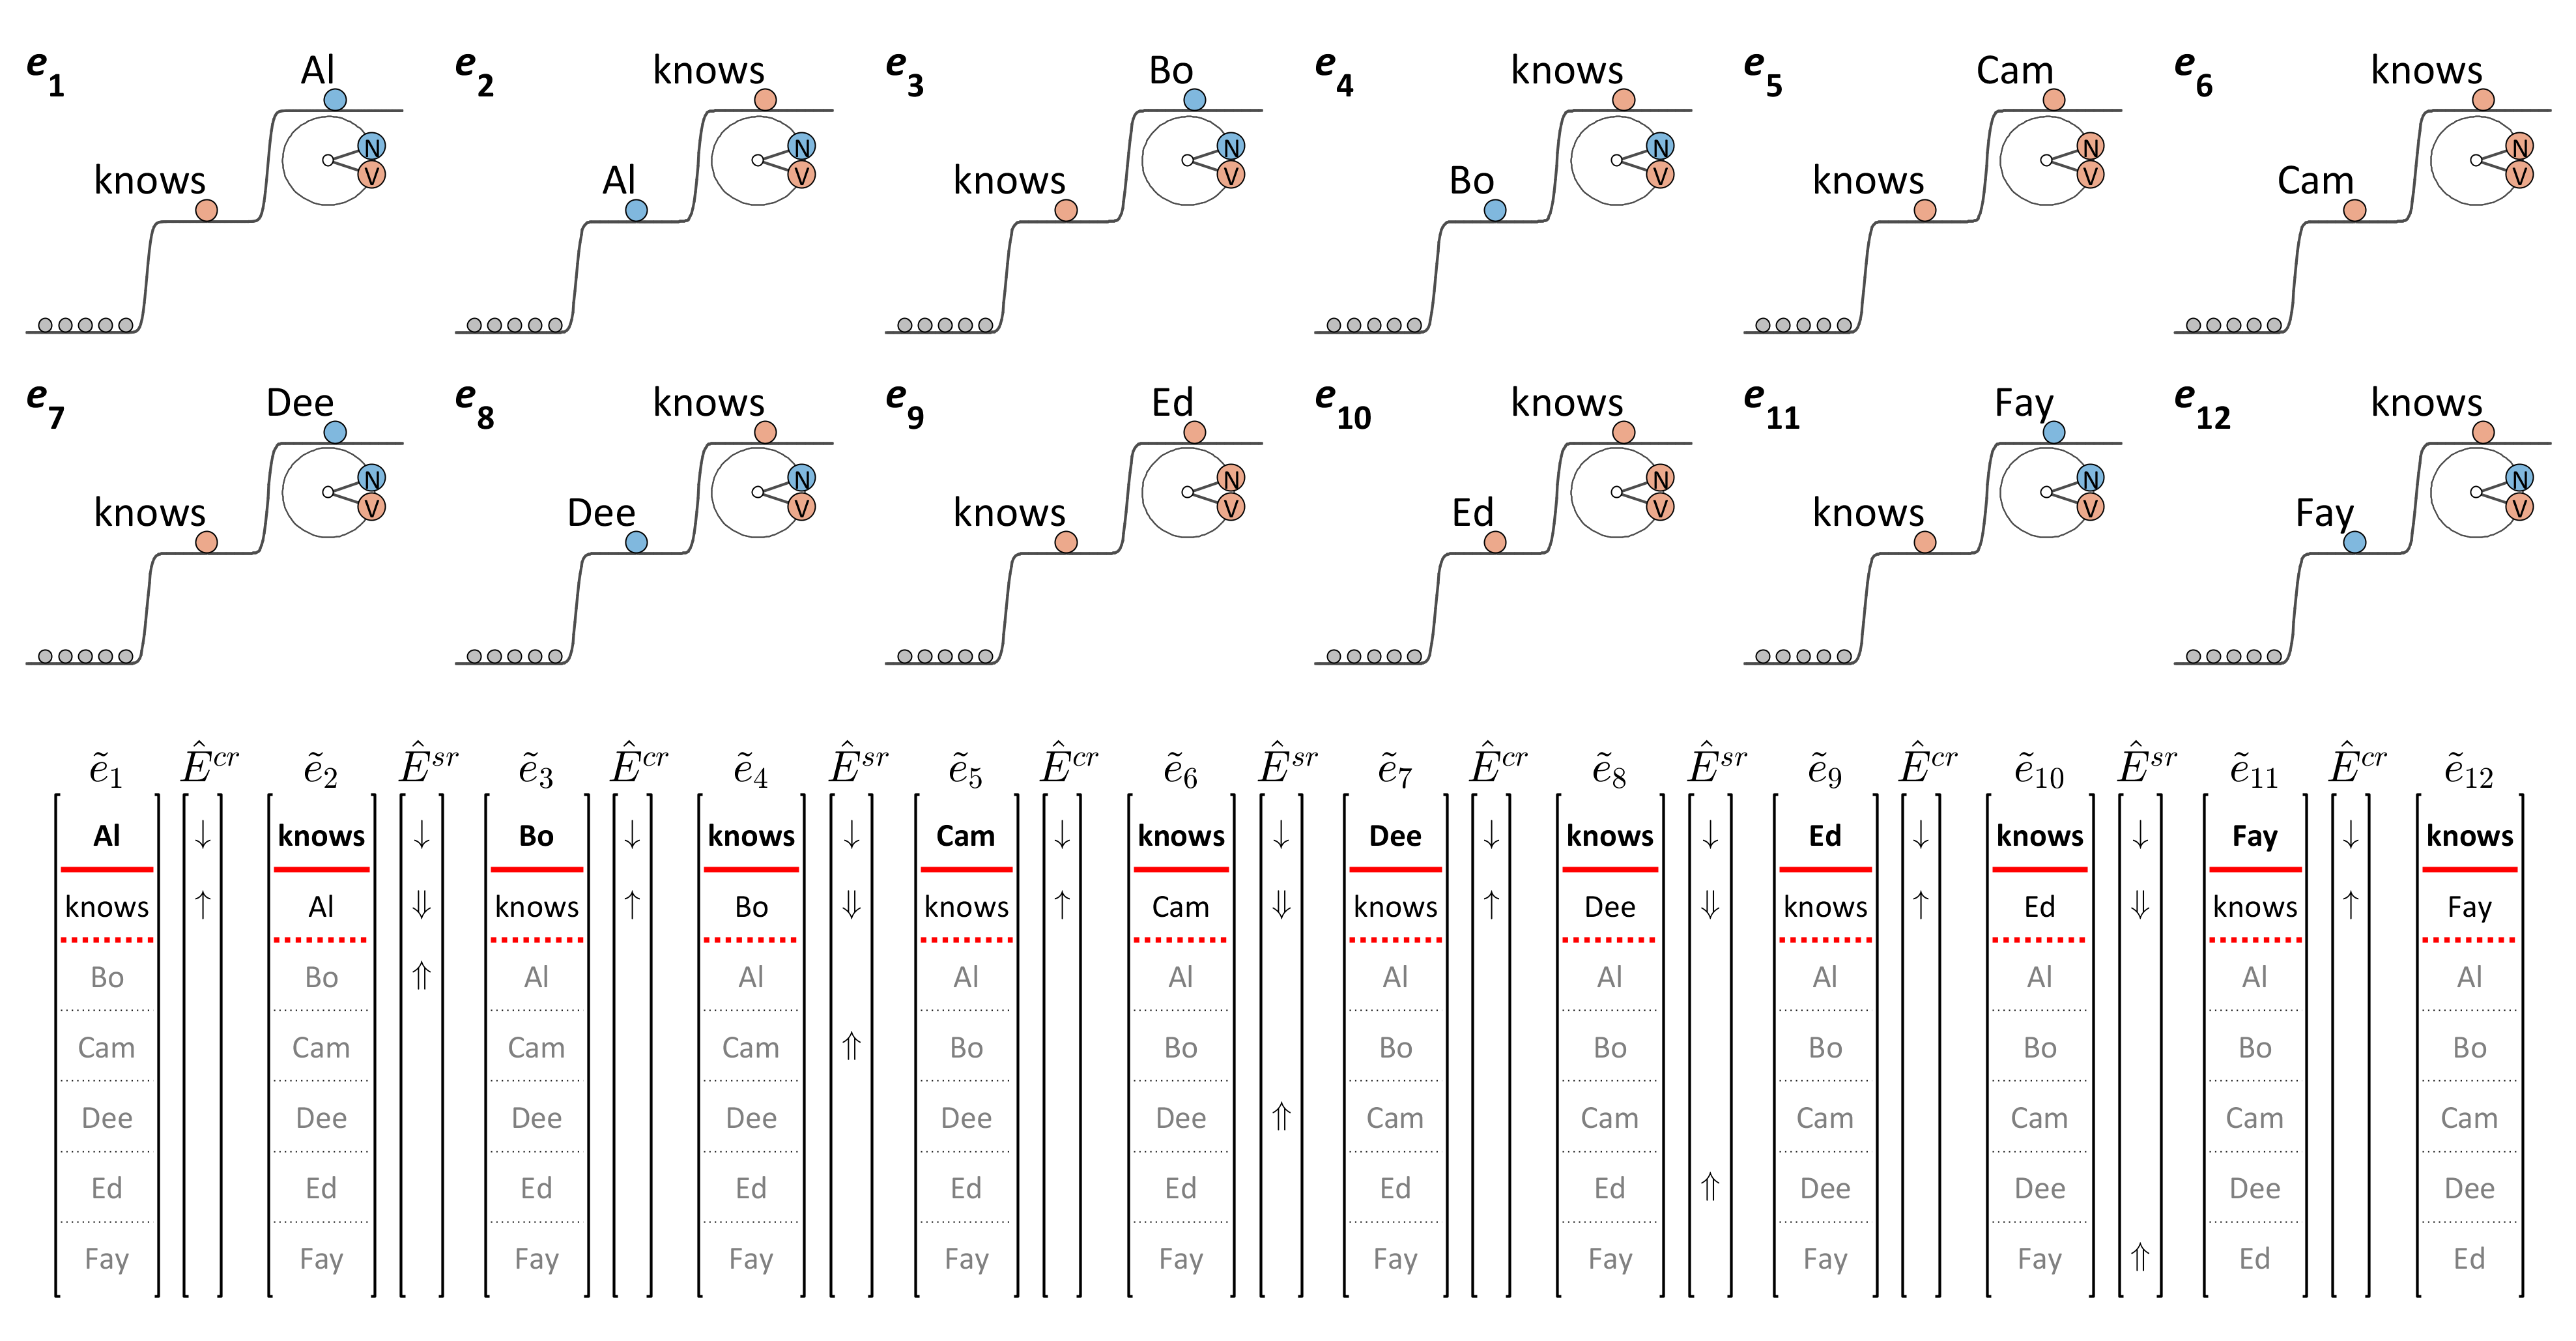
\includegraphics[width=\textwidth]{figures/Tilsen-img106.png}
\caption{A sequence of attended configurations does not imply co-presence.}
\label{fig:5:2}
\end{figure}
 

  There are two conventional objections that arise immediately from the rejection of co-presence. One is that o/el representations do not “represent” interclausal relational meanings. For example, when we say \textit{Al knows Bo drinks coffee}, our intuition is that there is a \isi{relational meaning} involving \textit{knows} and the \isi{complement clause}, i.e. that Al knows \textit{something} and the something that Al knows is the \isi{relational meaning} associated with \textit{Bo drinks coffee}. To represent interclausal \isi{relational meaning}, conventional approaches posit object-units such as S or CP, and connect these to other objects. Because of the connection/\isi{containment blend}, an S can represent the entirety of a clause in a single object. 

  The o/el response to this objection is that there is \textit{some} “relational” aspect of the experience of sequential attentional focus on {\textbar}Al knows{\textbar} and then {\textbar}Bo drinks coffee{\textbar}. But crucially, this experience is \textit{a very different sort of experience} than the experience of attending to a single-clause configuration such as {\textbar}Al drinks coffee{\textbar}. Whereas the {\textbar}Al drinks coffee{\textbar} experience corresponds to a stable ϕ-con\-fig\-u\-ra\-tion of excited systems, the experience of a “relation” between {\textbar}Al knows{\textbar} and {\textbar}Bo drinks coffee{\textbar} relies on a temporal juxtaposition of non-simultaneous experiences. Hence we cannot consider \textit{Al drinks coffee} and \textit{Al knows Bo drinks coffee} to be the same sort of trajectories. We should not conceptualize (or represent) the relation between {\textbar}Al knows{\textbar} and {\textbar}Bo drinks coffee{\textbar} in the same way as we conceptualize the relation between [Al]\{N\}, [drinks]\{V\}, and [coffee]\{V\}. Of course, connected object schemas do precisely that: treat interclausal relations as the same sort of relation as intraclausal ones.

  A second objection from the conventional perspective is that without an explicit configuration for \isi{interclausal meaning}, there is nothing to ensure that a producer attends to and produces configurations in the correct order, and nothing to ensure that an \isi{interpreter} is able to obtain an interpretation that matches the sequencing of attention of the producer. For example, without an explicit configurational mechanism for relating clauses, \textit{Al knows Bo knows Cam drinks coffee} could give rise to unintended interclausal relations, such as one in which Bo knows something that Cam knows. Indeed, this appears to happen. Interpreters are generally bad at keeping track of more than a couple of interclausal relational meanings evoked by an utterance. An \isi{interpreter} very well might misconstrue the interclausal relations from such an utterance. There \textit{is} (almost) \textit{no syntactic} mechanism to ensure that we experience the intended \isi{interclausal meaning} relations, other than temporal proximity. To remember an utterance such as above, a long-term memory mnemonic is helpful (e.g. alphabetically ordered proper names). In general, committing long sentences to memory -- i.e. a sequence of \isi{relational meaning} configurations -- involves associational mechanisms which are orthogonal to the organization of meaning experiences.

  The conclusion we reach is that \isi{interclausal meaning} relations cannot be conceptualized as experiences associated with a single configuration. Rather, interclausal meanings are associated with two or more configurations, which are attended in a sequence. Some reflection suggests that this conclusion may be more consistent with our intuitions than is generally appreciated. To what extent do you feel that your generic experiences of the main clause verbs in each of the columns of {\tabref{tab:5:1}} differ?

\begin{table}
\begin{tabularx}{\textwidth}{XX}
\lsptoprule
\textit{Bo knows something} & \textit{Bo knows that Al drinks coffee}\\
\textit{Cam believes in something} & \textit{Cam believes that Al drinks coffee}\\
\textit{Dee thinks something}  & \textit{Dee thinks Al drinks coffee}\\
\textit{Ed says something} & \textit{Ed says that Al drinks coffee}\\
\textit{Fay decides something} & \textit{Fay decides that Al drinks coffee}\\
\lspbottomrule
\end{tabularx}
\caption{Interclausal and intraclausal relational meaning experiences differ.}\label{tab:5:1}
\end{table}
  For many people, with a bit of careful reflection, these sets of experiences can be intuited to differ in a substantive way, which is nonetheless difficult to describe. The basis of this difference seems to be that the interclausal \isi{relational meaning} arises from the temporal proximity of configurations, whereas the intraclausal relational meanings are experienced simultaneously. One hint that \isi{interclausal meaning} is quite different from intraclausal \isi{relational meaning} is that verbs which take clausal complements are often verbs of cognition/communication (i.e. \textit{knows}, \textit{wants}, \textit{thinks}, \textit{believes}, \textit{says}, \textit{decides}, etc.). The fact that we can identify a semantic class of verbs with this behavior suggests that interclausal relations are not on par with intraclausal ones. 

  It is also relevant to the dissociation of inter- and intra-clausal meaning experiences that clausal “linkage” can be considered a phenomenon in and of itself, meriting typologies (\citealt{Bickel2010,Bril2010,Lehmann1988,VanValinJr1984}). Indeed, it is no accident that most of the interesting dependency phenomena necessarily hinge on dependencies between units associated with separate clauses. This is an important clue that intra- and inter-clausal meaning relations are fundamentally different phenomena.

  For the sake of conforming all meaning relations to the same image schematic structure, conventional theories construct categories like S and CP as if these are the same sort of entities as N or V. Such equations are misleading, in the o/el view. Our experience of interclausal \isi{relational meaning} differs substantially from our experience of intraclausal \isi{relational meaning}, thereby calling into question the conventional assumption in which all sorts of meaning relations are structurally homogenous.

  As far as the \isi{infinite set conception} is concerned, the consequence of rejection of co-presence of clausal meaning experiences is that we cannot collect an arbitrarily large number of utterances into a set, because those utterances are not the same sort of thing. Since we understand \textit{Bo knows Al drinks coffee} to be a different sort of phenomenon than \textit{Al drinks coffee}, it does not make sense to collect both into a set. Recall the natural numbers set construction discussed above, where we observed that adding the quasi-number 1* was undefined. Likewise, the sentence \textit{Al drinks coffee} is an S, a stable ϕ-con\-fig\-u\-ra\-tion, but the sentence \textit{Al knows Bo drinks coffee} is a quasi-sentence S*, a sequence of stable ϕ-con\-fig\-u\-ra\-tions. It is simply undefined to collect both of these into set. Put another way, if we wish to add a pebble to our bag, the whole pebble has to be \textit{there}, as a coherent system state, independent of time. We cannot add a quasi-pebble to our bag, because the quasi-pebbles are only partly there at any given time, and hence are not the same sort of thing as pebbles. In other words, phenomena which involve a temporal sequence of stable states cannot be reduced to \isi{atemporal} meta-con\-fig\-u\-ra\-tions.

  Even though we reject the notion of an infinite number of configurations, we might nonetheless conclude that there is an \isi{infinite set} of trajectories in \isi{state space}. This is not correct, or is correct in only a trivial way. Recall that the \isi{state space} itself is an analytical construct. This means that we construct the \isi{state space} to suit our needs for conceptualizing linguistic patterns. This space does not “exist” outside of a given analysis. Moreover, we allow for the dimensions of the space to change \textit{during} production or interpretation. This is useful for analyzing activation and de-activation of systems, i.e. the emergence and decay of collective oscillations in populations. It is also useful for analyzing \isi{surroundings} forces which are associated with peripheral \isi{sensorimotor} systems and other changes in the central nervous system. (Only in the canonical trajectory do we assume an invariant \isi{state space} throughout production.) The inherent temporality of our analysis space renders notions of \isi{infinity} meaningless: it is trivially true that we can never finish enumerating all of the possible trajectories, because the space itself can be constructed in infinitely many ways and because the trajectories do not have well defined beginnings and ends.

\section{The recursive conception of language}

The concept of a “\isi{narrow language faculty}” as a capacity for discrete \isi{infinity} derives from the construct of a “recursive” \textsc{Merge} operation, or a \isi{phrase structure} grammar. Recursion in language is controversial, and commentators both for and against the recursive view generally acknowledge a lack of clarity in what \textit{recursion} does or should refer to in this context (\citealt{Lobina2011,PullumScholz2010,Tomalin2011,vanderHulst2010}). So, what does it mean to say that \textsc{Merge} is “recursive”? Here I focus on two related notions of \isi{recursion} (see also \citealt{Tomalin2011}, who identifies nine different uses of \textit{recursion}). One has to do with how categories are defined: a \isi{syntactic category} like a sentence can be “recursive” if the sentence is defined such that it may “contain” or “connect to” another sentence. The other has to do with how rules or procedures can be applied: \isi{recursion} occurs when a procedure is applied to its own output. Below we discuss why neither of these is particularly appropriate for describing language, and we show how both rely on object metaphors with connection/containment schemas.

\subsection{Definitional recursion}

In some discussions of linguistic \isi{recursion}, the recursive nature of language is viewed as a consequence of including an object in its own definition. For example, when one defines a sentence as “a structure which optionally includes another sentence”, one refers to a sentence in its own definition. Notice the importance of structure here: what \textit{is} this “structure”? If it is a physical structure, how do we observe it? If it is a metaphorical structure, then what do we mean when saying that a “structure” “includes” another “structure”? The only sensible interpretation of such statements involves the \isi{object metaphor} and spatial schemas. For example, rewrite rules such as those in {\tabref{tab:5:2}}, provide directly and indirectly recursive definitions of sentences, but necessarily evoke \isi{object metaphor} conceptualizations because of the metaphor \textsc{symbols are objects}.

\begin{table}
\begin{tabularx}{\textwidth}{XX}
\lsptoprule
directly recursive & indirectly recursive\\
\midrule 
S → NP V S & S → NP \isi{VP}

\isi{VP} →  V S\\
\lspbottomrule
\end{tabularx}
\caption{Directly recursive and indirectly recursive rewrite rules.}\label{tab:5:2}
\end{table}
  
  Conventional schemas for conceptualizing rewrite rules impose certain constraints on their form: there is a horizontal linear arrangement of symbols (objects), with no vertical dimension. This convention derives from conceptualizing linguistic units as objects which occupy space -- without the metaphor, there is simply no basis for the conventions.

  Definitional \isi{recursion} is also problematic because the concept of a “definition” is quite vague. What constitutes a definition? The \isi{phrase structure} rewrite rules above are “definitions” of a sort, but if one were to elaborate on how or why rewrite rules are definitions, and what that could even mean, one would inevitably resort to many of the concepts which underlie procedural \isi{recursion}.

\subsection{Procedural recursion and the merge schema}

The deeper notion of \isi{recursion} is procedural: \isi{recursion} is a temporal pattern in which the output of a function (or “procedure”, or “process”, or “transformation”, etc.) can be the input to that same function. This flavor of \isi{recursion} also applies to the directly and indirectly recursive rewrite rules above, where the arrow is the function and the symbols at its head/tail are inputs/outputs. To reason about functions we commonly use object-transformation schemas of the sort in {\figref{fig:5:3}}.

  
\begin{figure}
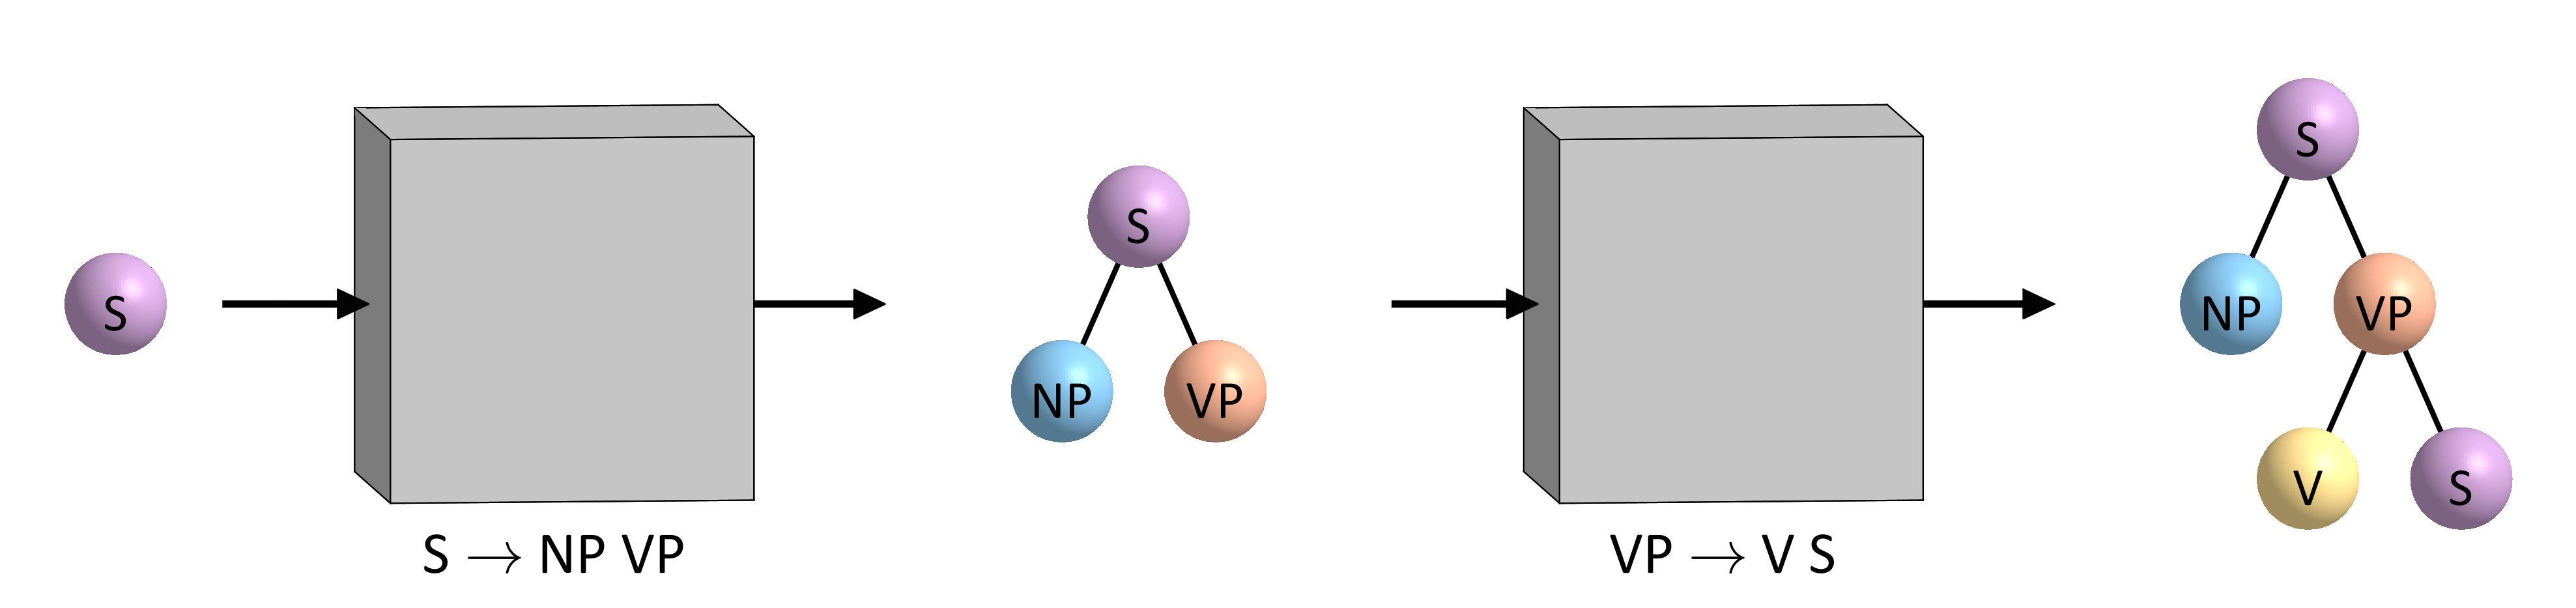
\includegraphics[width=\textwidth]{figures/Tilsen-img107.png}
\caption{Rewrite rules and the object-transformation schema.}
\label{fig:5:3}
\end{figure}
 

  In the \isi{object-transformation schema}, a function is a container, an object structure goes into the container, the object is transformed, and a new object structure comes out. For rewrite rules, the transformation is often such that some object in the input structure is split into new objects which are connected to it. The operations “external merge” and “\isi{internal merge}” are also object-transformation schemas. External merge takes two input objects, creates a new object (which is always a phrasal category), and connects them to the new object, as in {\figref{fig:5:4}}. Internal merge, as shown in {\figref{fig:5:5}}, transforms a structure of objects by (i)~disconnecting an object from the structure and (ii) externally merging the remaining structure of objects with the disconnected object, again creating a new phrasal object. In both cases, exactly the same connected-object schemas are used for inputs and outputs. Hence the input structures are the same type of thing as the transformed, output structures. Moreover, input objects are never destroyed, so the structures can grow to infinite size.

  
\begin{figure}
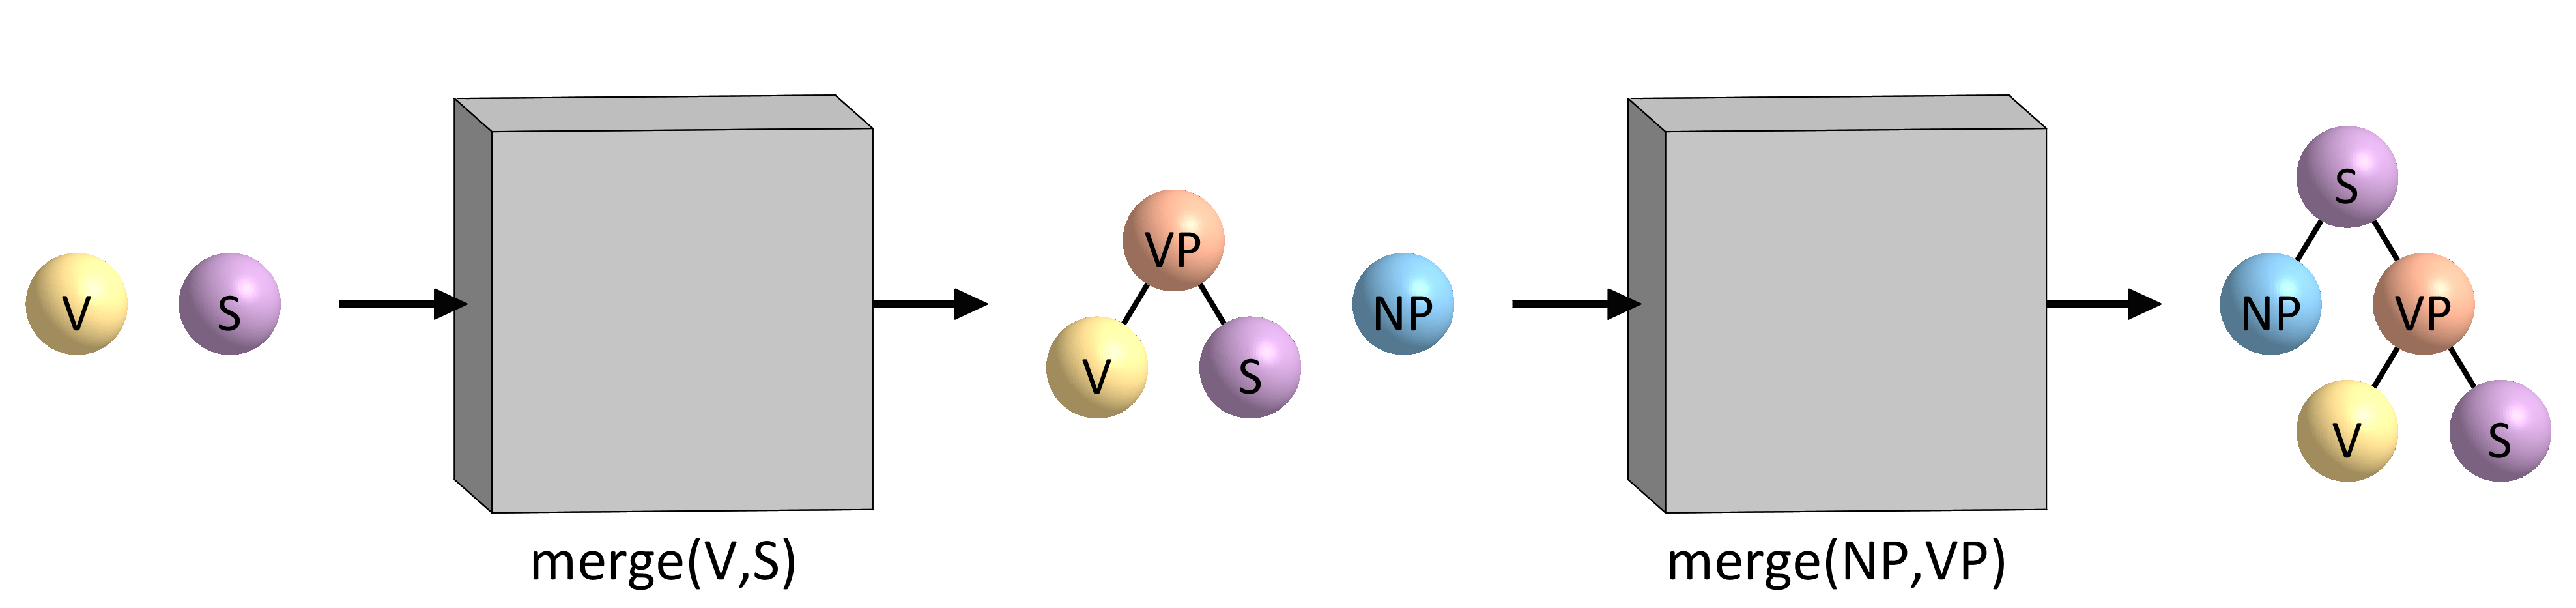
\includegraphics[width=\textwidth]{figures/Tilsen-img108.png}
\caption{Merge and the object-transformation schema.}
\label{fig:5:4}
\end{figure}
 
\begin{figure}
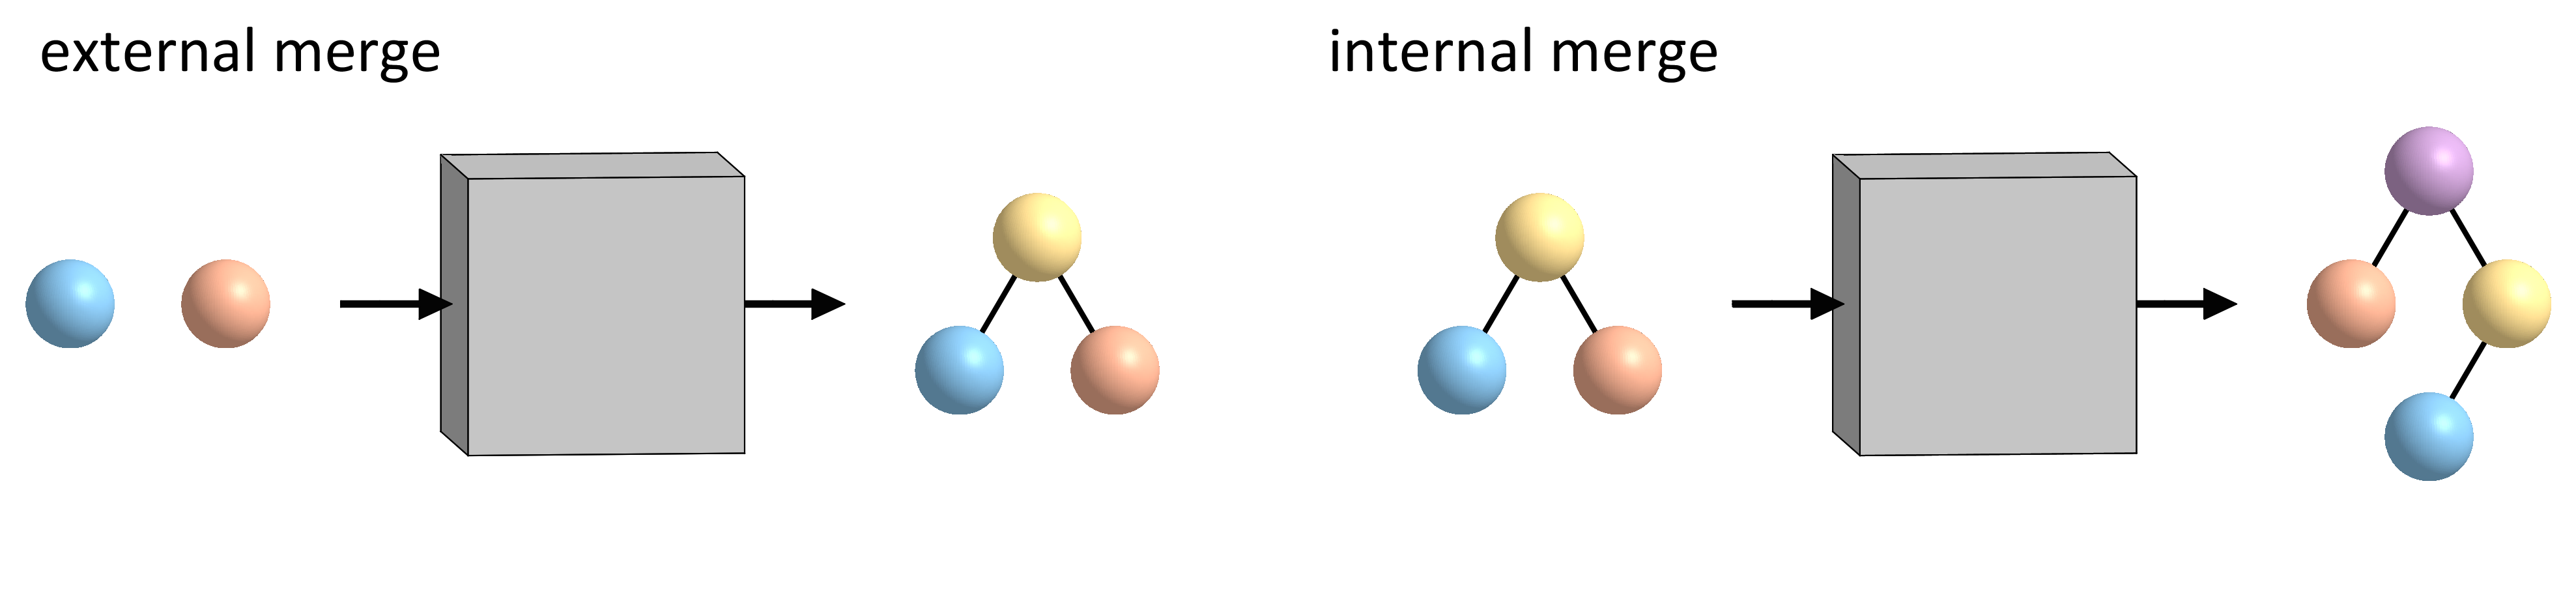
\includegraphics[width=\textwidth]{figures/Tilsen-img109.png}
\caption{Comparison of external and internal merge in the object-transformation schema.}
\label{fig:5:5}
\end{figure}

  By conceptualizing merge in this way, all linguistic structures are trivially recursive. The function (i.e. the narrow faculty of language, \textsc{Merge}), takes its own output as input. Notice that in both the rewrite and \textsc{Merge} variations, there are “parts” of the output structures that were also present in the input structures, and there is a new object/structure that is created. Recall from earlier discussion that the implicit temporal information in patterns of connection and orientation is what makes “internal” \textsc{Merge} necessary. Can we relate this observation to differences between external and internal variants of \textsc{Merge} in the function schema? Consider what has been written about these variants:

\begin{quote}
NS [\textit{narrow syntax}] is based on the free operation \isi{Merge}. SMT [\textit{the strong \isi{minimalist} thesis}] entails the \isi{Merge} of α, P is unconstrained, therefore either external or internal. Under external \isi{Merge}, α and P are \textbf{separate objects}; under internal \isi{Merge}, \textbf{one is part of the other}, and \isi{Merge} yields the property of “displacement,” which is ubiquitous in language and must be captured in some manner in any theory. It is hard to think of a simpler approach than allowing internal \isi{Merge} (a “grammatical transformation”), an operation that is freely available. Accordingly, displacement is not an “imperfection” of language; its absence would be an imperfection. \citep[8]{Chomsky2001b}
\end{quote}

  Internal \textsc{Merge} differs from external \textsc{Merge} in that it changes the \isi{spatial arrangement} of objects in one input structure. External \textsc{Merge} imposes a new \isi{spatial arrangement}/connection pattern on two “separate” input objects. The “separation” is a spatial relation associated with connection: the input objects, because they are not connected, are not spatially related. Both external and internal \textsc{Merge} create objects in the output which were not present in the input. 

  Note that \textsc{Merge} creates structure, but does not \textit{destroy} structure. Intriguingly, no structure destroying operation appears to be utilized in many conventional approaches. This analytic asymmetry follows from the object persistence mapping: objects which are present persist in time. Indeed, this is necessary for the procedural notion of \isi{recursion}, which is claimed to be the core property of language:

\begin{quote}
NS [\textit{narrow syntax}] has one operation that comes “free,” in that it is required in some form for any \isi{recursive system}: the operation \isi{Merge}, which takes two elements, α, P already constructed and creates a new one consisting of the two; in the simplest, \{α, P\}. The operation yields the relation of membership, and assuming iterability, the relations dominate (contain) and term-of. \citep[6]{Chomsky2001b}
\end{quote}

\begin{quote}
All approaches agree that a core property of FLN [\textit{narrow faculty of language}] is \isi{recursion}, attributed to \isi{narrow syntax} in the conception just outlined. FLN takes a finite set of elements and yields a potentially infinite array of discrete expressions. This capacity of FLN yields discrete \isi{infinity} (a property that also characterizes the natural numbers). \citep[1571]{HauserEtAl2002}
\end{quote}

\begin{quote}
Natural languages go beyond purely local structure by including a capacity for recursive embedding of phrases within phrases, which can lead to statistical regularities that are separated by an arbitrary number of words or phrases. Such long-distance, hierarchical relationships are found in all natural languages for which, at a minimum, a ``phrase-structure grammar" is necessary. It is a foundational observation of modern generative linguistics that, to capture a natural language, a grammar must include such capabilities. \citep[1577]{HauserEtAl2002}
\end{quote}

  There has never been, and likely will never be, a “recursive” conception of language which does not derive from the \isi{object metaphor}. Whether we use a term like “function”, “process”, “system”, “operation”, “mapping”, “transformation”, etc. is irrelevant, given that the inputs and outputs are understood as objects. \textsc{Merge} is procedural \isi{recursion} because it imposes objectness on its input and output, not because \textsc{Merge} has some \textit{essential property} of being recursive.

\subsection{\textsc{Merge} and the need for \textsc{Phases}}

One of the most remarkable ironies of the conventional program is that \textsc{Merge} and the \isi{object metaphor} give rise to entailments that, in order to be consistent with empirical observations, necessitate other, incompatible entailments associated with the concept of \textsc{\isi{minimalist} Phase} (\textsc{\citeauthor{Chomsky2001b} \citeyear*{Chomsky2001b,Chomsky2008}}). That \textsc{Merge} requires conceptual structures which are incompatible with itself is not surprising: the conceptual structures of any theory predetermine its inherent contradictions.

  To see the contradictions, let's consider the entailments of \textsc{Merge} and the \isi{object metaphor} in more detail. The connected object structures in {\figref{fig:5:6}} encourage us to see substructures \textit{within} larger structures, i.e. “parts” of the structure can be identified, and these parts are \textit{within} the structure. For such representations to make sense, we must: (i) view all parts of a structure as \textit{there} at the same time, i.e. as \textit{co-present}; (ii) view the presence of any part as \textit{equivalent to} the presence of any other part; and (iii) assume an infinite amount of space for the structure. Below we examine each of these assumptions.
  
\begin{figure}
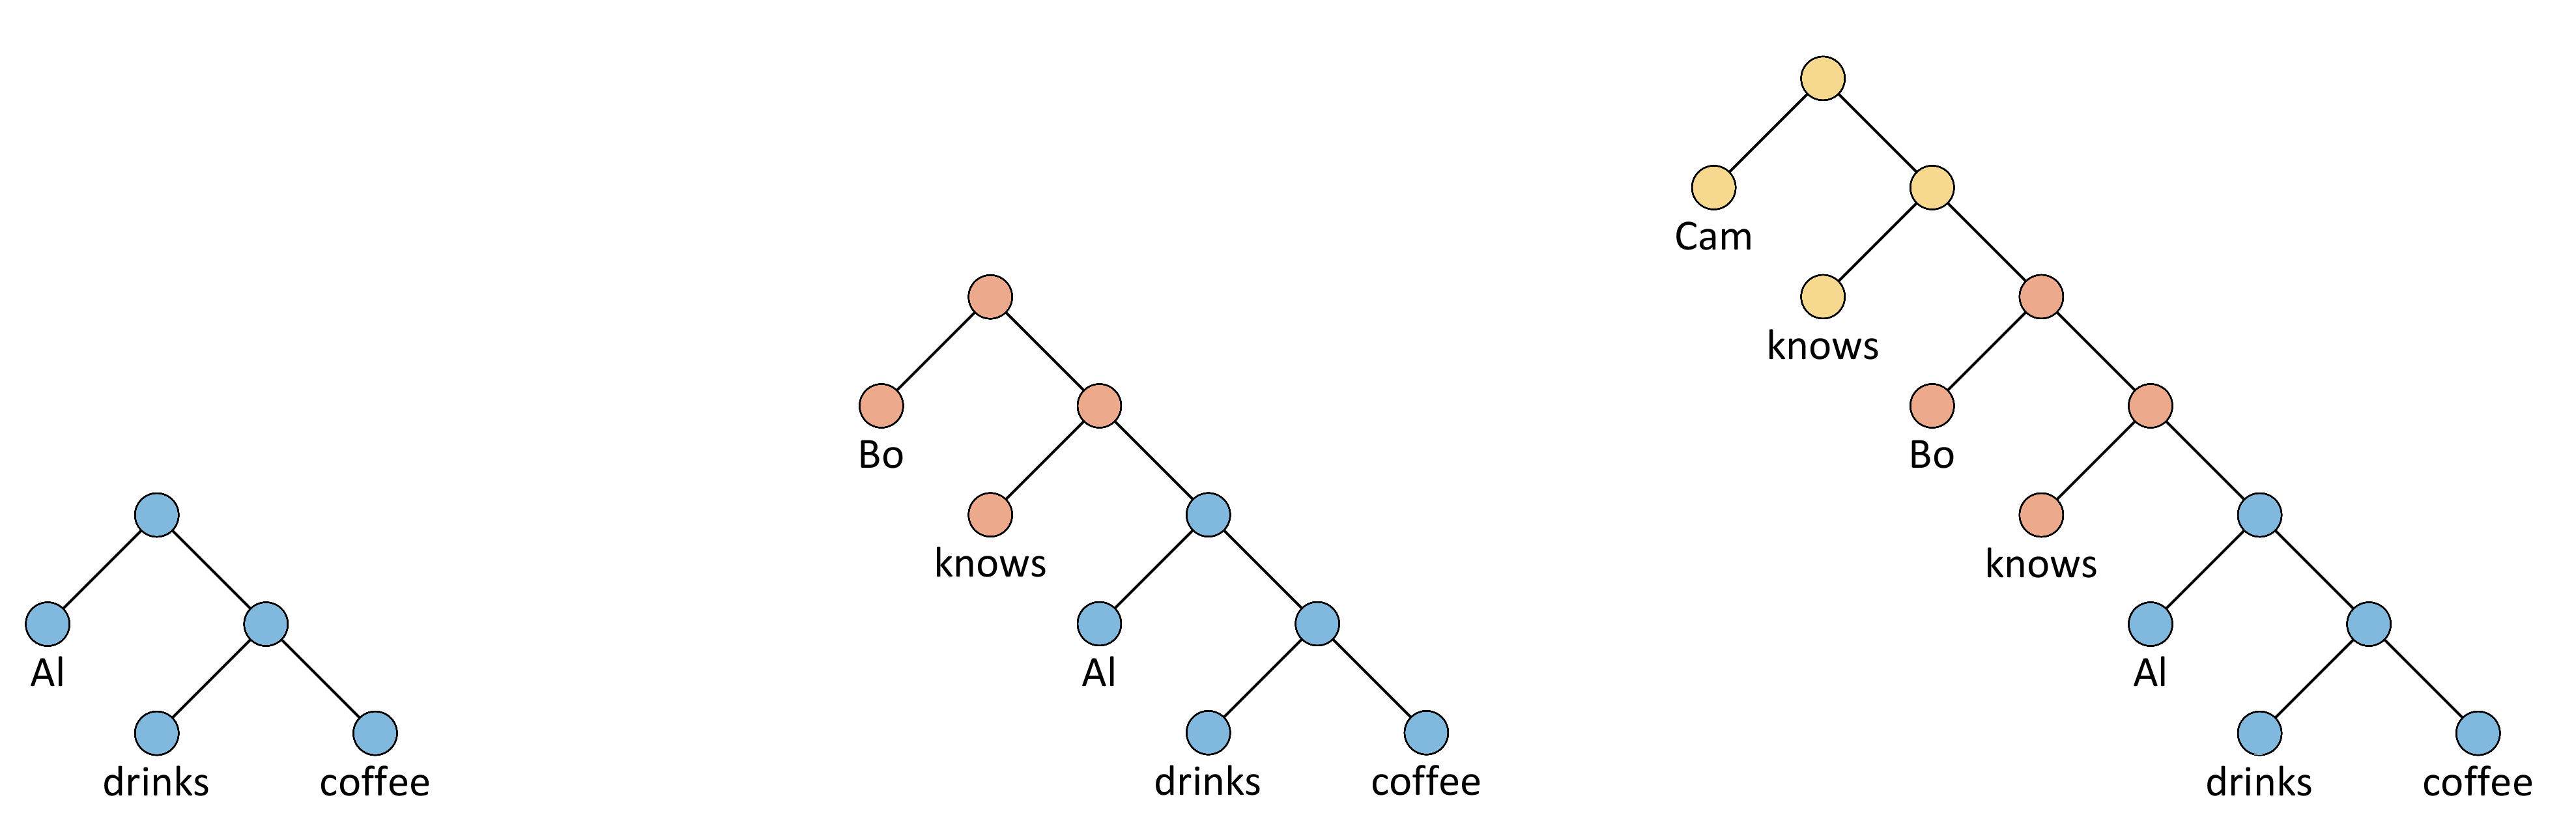
\includegraphics[width=\textwidth]{figures/Tilsen-img110.png}
\caption{Conventional representions depict all substructures as equally co-present.}
\label{fig:5:6}
\end{figure}
 

(i) \textit{Co-presence of structure}: the entirety of the structure is simultaneously present. The \isi{object metaphor} allows us to view all of the “structure” as \textit{present}, simultaneously. In other words, there is a moment in time when all of the syntactic systems and associated concepts, as well as their relations (connections) are \textit{there}, in space. Should we ask where “there” is? One interpretation is that spatial presence corresponds to some sort of cognitive attention. Attention to a \isi{linguistic unit} is the spatial presence of that unit. Hence there is an existence entailment that comes merely from depicting the structure as co-present in a region of space and time, and this in turn entails simultaneous attention to a set of units.

  Note that we can readily distinguish co-presence from co-origination. The co-presence of structure does not imply that all of the substructures in the larger structure came into being at one time. Likewise, co-presence does not imply co-termination: we can make no inferences about what happens to the structure or its parts after it is built. It is easy to ignore, but the co-presence inference leaves many open questions: where do the objects and their relations come from, where do they go? How long are they present? What is the nature of the space they occupy?
  
  Of course, one might reject the notion that presence of the entirety of a structure in conventional representations entails simultaneous and commensurate attention to the whole structure. But this stance begs the questions of which parts of the structure are attended to and in what order those parts are attended to. Connected-object structures do not explicitly convey this information. In contrast, representations in the o/el framework very directly provide this information.

(ii) \textit{Equivalence of structural presence:} the presence of any part of the structure is equivalent to the presence of any other part. The \isi{object metaphor} entails this equivalence. Recall that the procedural \isi{recursion} of \textsc{Merge} arises simply because input and output are the same sort of thing -- syntactic objects -- they are equivalent in this sense. The metaphor does not allow for distinctions to be drawn in the degree to which parts of the structure are present. In the above example, one cannot say that \textit{Cam knows} and the structure of \textit{Al drinks coffee} are differently present. Structural presence is necessarily dichotomous: objects and relations are either there or not there, never partially there. There is no privileged part of the structure that is “more present” than other parts, in time or in space. Hence if we substitute \textit{presence} with \textit{attention to meaning relations}, object representations do not allow for temporal variation in the \textit{degree} of attention to any subset of relations associated with an utterance. 

(iii) \textit{Infiniteness of space:} the space for a connected-object structure is infinite. \textsc{Merge} requires this, because objects occupy space, and objects cannot occupy the same space. So, the more objects that are “present” in a structure, the more space is occupied by the entire structure. This space is, generally, a volume (often shown as two-di\-men\-sional). Imposing limits on the space would be quite arbitrary. Where would these limits come from? Certainly there is no intuitive source for such limits if the language faculty is isolated from all other cognitive systems. Infinite space seems problematic if structural presence has any cognitive relevance whatsoever. Under the attentional metaphor (attention to a \isi{linguistic unit} is the spatial presence of that unit), infinite space implies infinite attention, which is nonsensical. Consider the sentence (from George Bernard Shaw) that Pinker chose to illustrate the “infinite capacity” of language:

\begin{quote}
Stranger still, though Jacques Dalcroze, like all these great teachers, is the completest of tyrants, knowing what is right and that he must and will have the lesson just so or else break his heart (not somebody else’s, observe), yet his school is so fascinating that every woman who sees it exclaims: ‘Oh why was I not taught like this!’ and elderly gentlemen excitedly enroll themselves as students and distract classes of infants by their desperate endeavours to beat two in a bar with one hand and three with the other, and start off on earnest walks around the room, taking two steps backward whenever Monsieur Dalcroze calls out ‘Hop!’ \citep{Pinker2003}.
\end{quote}

  If we describe the passage above as “a sentence”, then the word “sentence” is mostly useless for analytical purposes. Indeed, we might as well characterize the entire Shaw novel as “a sentence”, or all of the novels that Shaw ever wrote, or all that has ever been written and spoken by anyone: all of the syntactic objects that have been combined by \textsc{Merge} remain \textit{there}, co-present and equivalent, occupying infinite space. 

  Clearly we should reject the entailments of co-presence, equivalence of structure, and infiniteness of space in such examples, because it is obvious that our brains cannot simultaneously attend to the entirety of such “sentences”. Reflect on what happens when you try to interpret the following, more constrained example:

\ea
\textit{Fay knows Ed knows Dee knows Cam knows Bo knows Al drinks coffee.}
\z

  Do you attend to all of the relational meanings evoked by the utterance at the same time? Doubtful. As you read the sentence, new relational meanings are excited while previous ones are suppressed. Even after you have read the sentence, comprehending it seems to involve cycling through a series of relational meanings, rather than achieving some sort of holistic state. The experience of meaning in so-called recursive utterances is not temporally uniform. Connected object representations provide no explanation for why our attention is limited to relatively short “pieces” of such sentences, such as those shown in {\figref{fig:5:7}}. The entailments of \textsc{Merge} prevent us from reasoning about why there might be limitations on the sizes of these pieces.

  
\begin{figure}
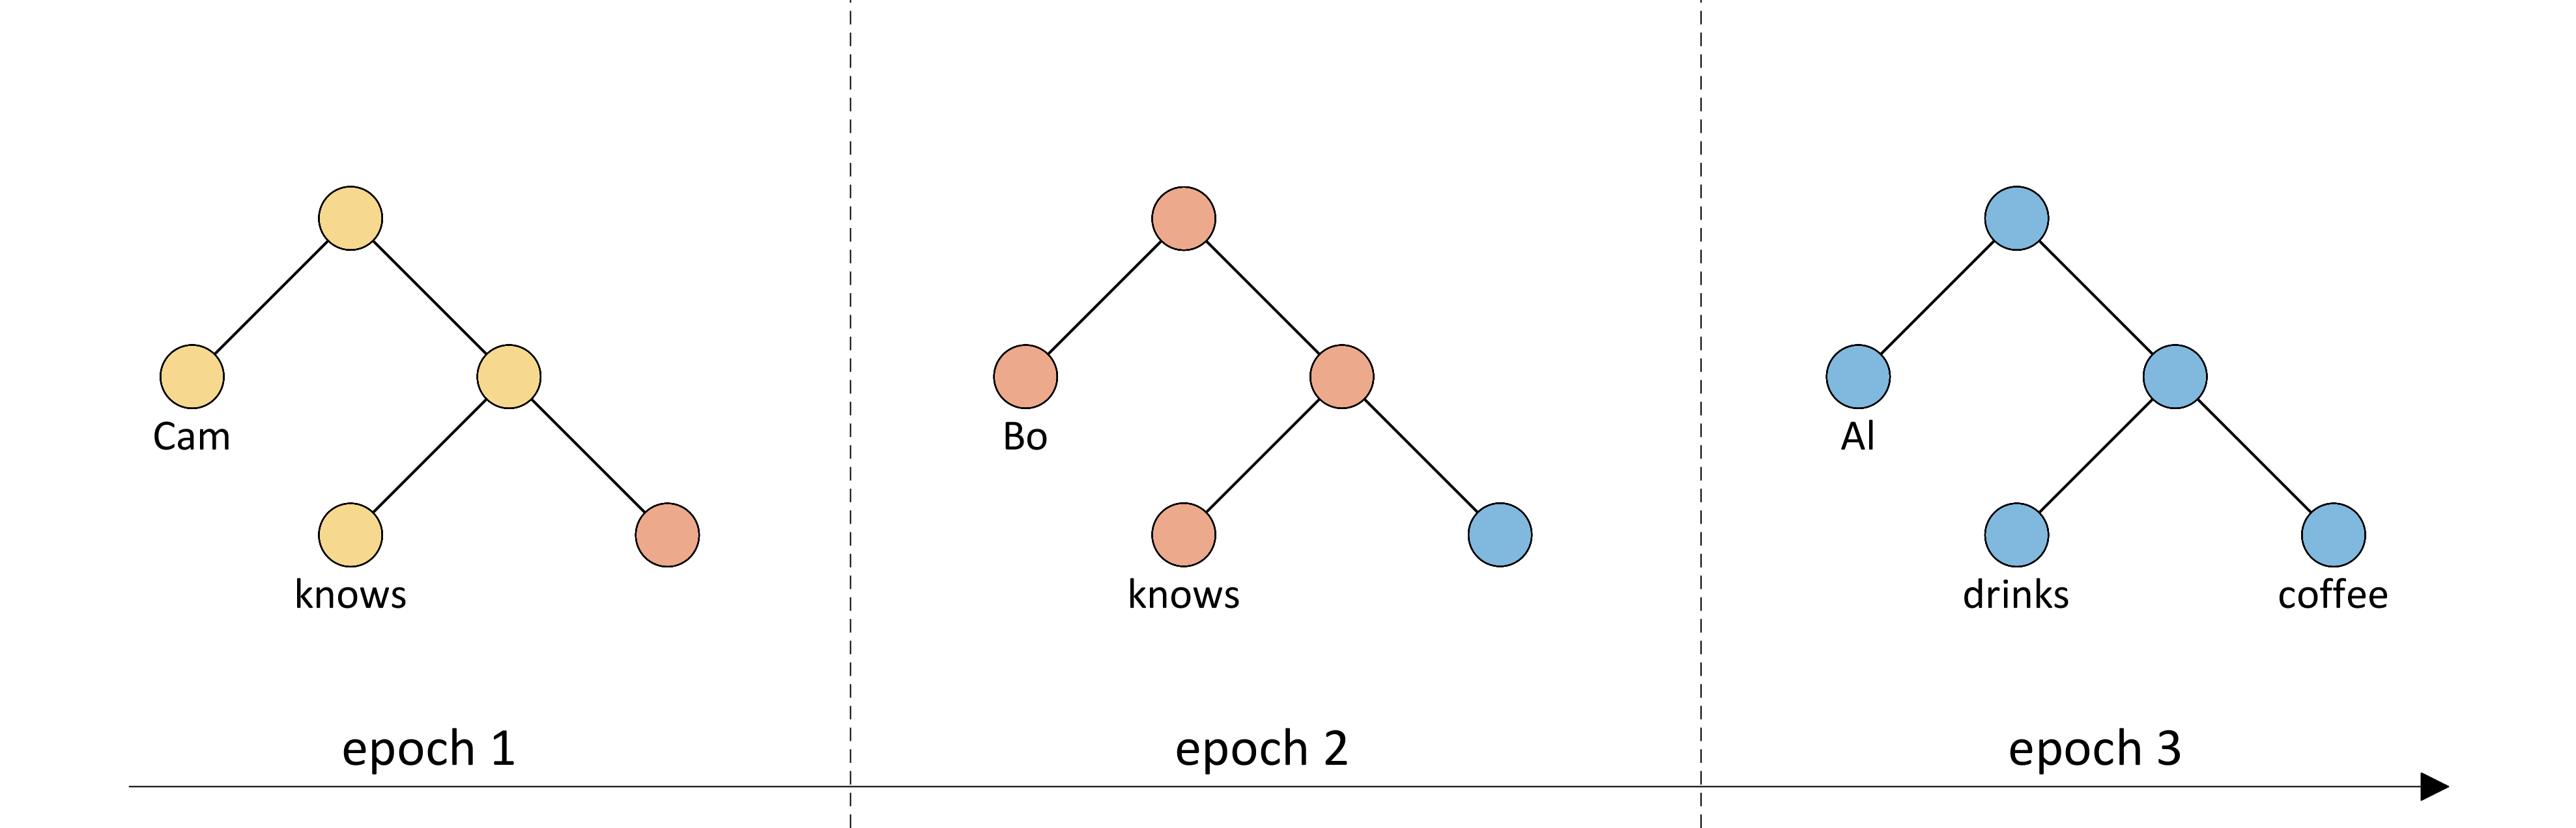
\includegraphics[width=\textwidth]{figures/Tilsen-img111.png}
\caption{A sequence of relational meaning experiences represented with disconnected structures.}
\label{fig:5:7}
\end{figure}
 

  The conventional rhetoric to address the mismatch between theory and intuition is to construct an unhelpful isolation of “the \isi{narrow syntax}” from “external interfaces,” i.e. \isi{sensorimotor} and conceptual-intentional systems. The external interfaces are held responsible for the attentional limitations, and without them, \textsc{Merge} would happily create infinitely large structures. 

  This sort of compartmentalizing, of \isi{narrow syntax} vs. other systems, is not a useful strategy for advancing our understanding. Problematically, it necessitates the \isi{minimalist} concept of a \textsc{Phase}, which is ultimately a mechanism for \textit{separating} connected object structures into pieces (or preventing the pieces from becoming too large in the first place). Minimalist \textsc{Phases} thereby restrict what sorts of objects \textsc{Merge} can operate on. Consider the following description:

\begin{quote}
For minimal computation, as soon as the information is \textbf{transferred} it will be \textbf{forgotten}, not accessed in subsequent stages of derivation: the computation will not have to \textbf{look back at earlier phases} as it proceeds, and cyclicity is preserved in a very strong sense. Working that out, we try to formulate a \textit{phase \textit{impenetrability} condition} PIC, conforming as closely as possible to SMT. \citep[9]{Chomsky2008} [emphasis added]
\end{quote}

  There are several rich metaphors in the above passage. The notion that information (i.e. structure) is “transferred” implies two spaces, with motion of structure to and from those spaces. The notion that a space can be “impenetrable” reinforces the separation schema imposed by \textsc{Phases}; the schema evokes a \textit{barrier}. Moreover, the notion that a computation may “look back” at “earlier phases” evokes a spatial schema for time, and this is blended with the metaphor that computation is human perception and action. The processes which drive change in brain states -- so-called “computations” -- are described as if there are animate agents who attend to objects in space and manipulate them.

  Even if these metaphors were more useful than misleading, the problem with \textsc{Phases} is that they lead to somewhat bizarre explanations, which are ultimately not compatible with the entailments of \textsc{Merge}. Let's compare two patterns,\linebreak which are understood to have the same number of \textsc{Phases}, but which differ with regard to the \isi{acceptability} of related \textit{Wh}-object questions:

\ea\label{ex:5:x1}
\ea{Bo knows \textbar{} that Al drinks coffee.}
\ex{What does Bo know \textbar{} that Al drinks?}
\z
\z

\ea\label{ex:5:x2}
\ea{Bo wonders \textbar{} if Al drinks coffee.}
\ex{*What does Bo wonder \textbar{} if Al drinks?}
\z
\z

\textsc{Phases} play a role in some accounts of why the \textit{Wh}-question in \REF{ex:5:x1} is acceptable while the one in \REF{ex:5:x2} is not. In both examples, the two clauses of the sentences are different \textsc{Phases}. The Wh-object is assumed to be generated in the embedded clause and must move out of that clause. The “movement” from one phase to another is argued to be possible only when the \textit{Wh}-object can move to a particular position in the structure, an “escape hatch” so to speak. This location of the “escape hatch” is held to be occupied in \REF{ex:5:x2}, but not in \REF{ex:5:x1}, and hence the Wh-object can only move out of the \textsc{Phase} in \REF{ex:5:x1}. Now consider sentences such as those in \REF{ex:5:x3} and \REF{ex:5:x4}: 

\ea\label{ex:5:x3}
\ea{Jo knows \textbar{} Irv knows \textbar{} Hal knows \textbar{} Guy knows \textbar{} Fay knows \textbar{} Ed knows \textbar{} Dee knows \textbar{} Cam knows \textbar{} Bo knows \textbar{} Al drinks coffee.}\label{ex:5:x3a}
\ex{What does Jo know \textbar{} Irv knows \textbar{} Hal knows \textbar{} Guy knows \textbar{} Fay knows \textbar{} Ed knows \textbar{} Dee knows \textbar{} Cam knows \textbar{} Bo knows \textbar{} Al drinks?}\label{ex:5:x3b}
\z
\z

\ea\label{ex:5:x4}
\ea{Jo wonders \textbar{} if Irv wonders \textbar{} if Hal wonders \textbar{} if Guy wonders \textbar{} if Fay wonders \textbar{} if Ed wonders \textbar{} if Dee wonders \textbar{} if Cam wonders \textbar{} if Bo wonders \textbar{} if Al drinks coffee.}\label{ex:5:x4a}
\ex{*What does Jo wonder \textbar{} if Irv wonders \textbar{} if Hal wonders \textbar{} if Guy wonders \textbar{} if Fay wonders \textbar{} if Ed wonders \textbar{} if Dee wonders \textbar{} if Cam wonders \textbar{} if Bo wonders \textbar{} if Al drinks?}\label{ex:5:x4b}
\z
\z

  In both sentences, the “computation” never “looks at” the entirety of the utterance. In \REF{ex:5:x3b} the \textit{Wh}-object is able to move out of each phase, one after the other (a total of 9 movements), but not so for \REF{ex:5:x4b}. More abstractly, in \REF{ex:5:x3b} the computation looks at a particular position in a particular structure X1, which corresponds to a part of the sentence (e.g. \textit{Al knows}). The computation then allows an object in that particular position of structure X1 to “move” to a separate structure, X2 (\textit{Bo knows}), which is never connected to X1. The object can be passed through escape hatches in each \textsc{phase}: X3 (\textit{Cam knows}), X4 (\textit{Dee knows}), etc., and all of these structures are never connected to each other.
  
    These absurd descriptions of the difference between the sentences in \REF{ex:5:x3} and \REF{ex:5:x4} show that the entailments of \isi{minimalist} \textsc{phases} are inconsistent with the entailments of \textsc{Merge}. The connected objects which \textsc{Merge} produces are co-present, and these should be available as input to \textsc{Merge} (in particular, to internal \textsc{Merge} in the case of \textit{Wh}-islands). \textsc{Phases} prevent \textsc{Merge} from operating on the entirety of a sentence by separating it into pieces. This leads to numerous oddities: \textsc{Phases} attempt to preserve co-presence for parts of a structure, but in effect abandon global co-presence; they attempt to preserve \isi{atemporality} for pieces of the structure, but impose temporality on complex sentences; they attempt to preserve uniform spaces for subsets of objects in a sentence, but divide sentences into mutually inaccessible spaces for each subset. The theme here -- preserving some form of local homogeneity of structure while abandoning homogeneity between epochs -- is exactly what we accomplish in the o/el framework, only far more straightforwardly and without creating theory-internal contradictions. Instead of \textsc{Merge}, the basic operations are \textsc{Couple} and \textsc{Reorganize}.

  The crux of the incompatibility between \textsc{Merge} and \textsc{Phases} can be demonstrated by considering how the glorified claims of recursive \textsc{Merge} become much less powerful when modified to allow for the entailment that different \textsc{Phases} are different spaces for objects. Here is the previous description of \textsc{Merge}, with my modifications in bracketed bold text:

\begin{quote} 
NS has one operation that comes “free” \textbf{[for each space of objects]}, in that it is required in some form for any \textbf{[space-limited]} \isi{recursive system}: the operation \isi{Merge}, which takes two elements \textbf{[in the same space of objects]}, α, P already constructed and creates a new one \textbf{[in that space]} consisting of the two elements; in the simplest, \{α, P\} \textbf{[given space ψ]}. The operation yields the relation of membership, and assuming iterability \textbf{[in space ψ]}, the relations dominate (contain) and term-of. (\textit{modified from} \citep[6]{Chomsky2001beyond})
\end{quote}

  The modified description of \textsc{Merge} begs the question of why should there be \textsc{Phases} at all? The consequences of the profound conflict between \textsc{Phases} and \textsc{Merge} do not seem to have been acknowledged in much of the literature on \textsc{Phases}. The crux of the problem is that \textsc{Merge} entails that output structures are one structure, but this runs contrary to the spatial separation that \textsc{Phases} impose in various circumstances. It is important to emphasize that \textsc{phases} are necessary in the first place, because there is something wrong with \textsc{Merge}. \textsc{Merge} is problematic \textit{because} it is a recursive operation on \textit{objects}. Language is not a structure of objects.

\section{Recursion as state similarity}

If language is not a structure of objects generated by a recursive procedure, is there an alternative way to conceptualize the difference between utterances\linebreak which, in the conventional sense, would be considered “recursive”, from those which would be considered “non-recursive”? Can we distinguish recursive patterns (e.g. \textit{Cam knows Bo knows…}) from non-recursive ones (e.g. \textit{Cam knows something. Bo knows something}) in the o/el conception? 

  In recursive sentences, the state trajectory returns to a location in \isi{state space} that is similar to (i.e. near to) a previous state, given some arbitrary conditions on similarity, the timescale of the return, and intervening states. Note that in the conventional perspective, the conceptual dimensions of recursive utterances are considered irrelevant vis-à-vis \isi{recursion}, and only the syntactic dimensions matter. Hence \textit{Cam knows Bo suspects…} is just as recursive as \textit{Cam knows Bo knows}..., because both have the syntactic unit pattern [N V [N V…]]. Our analysis below adopts the same imposition. Hence we can view \isi{recursion} simply as the return of a system state to a previously visited location in \isi{state space} (or at least a return to some location which is “near” to a previously visited one). This interpretation of \isi{recursion} is consistent with \isi{connectionist} models which accomplish the generation or interpretation of “recursive” patterns (\citealt{ChristiansenChater1999,Elman1989,Smolensky1990}).

\subsection{Recursion as temporally disjoint but similar system states}

To exemplify the o/el conception of \isi{recursion}, we consider a sequence of s-sys\-tem ϕ/e-state vectors for the utterance \textit{Cam knows Bo knows Al drinks coffee}, shown in {\figref{fig:5:8}}. Each element of the vector corresponds to an s-sys\-tem state. The state is represented by an integer whose magnitude is the e-level and whose sign indicates whether the system is ϕ-proximal or distal relative to the main clause \{V\}. Notice that a state in which there is a highly excited \{+N\} system and a highly excited \{V\} system occurs in three epochs (e1, e3, e5). Although these s-sys\-tem states are not identical, they are similar, and thus relatively close to each other in the \isi{state space}. We can thus think of \isi{recursion} as the return of the state trajectory to a \isi{state space} location near to a previously visited one.

  
\begin{figure}
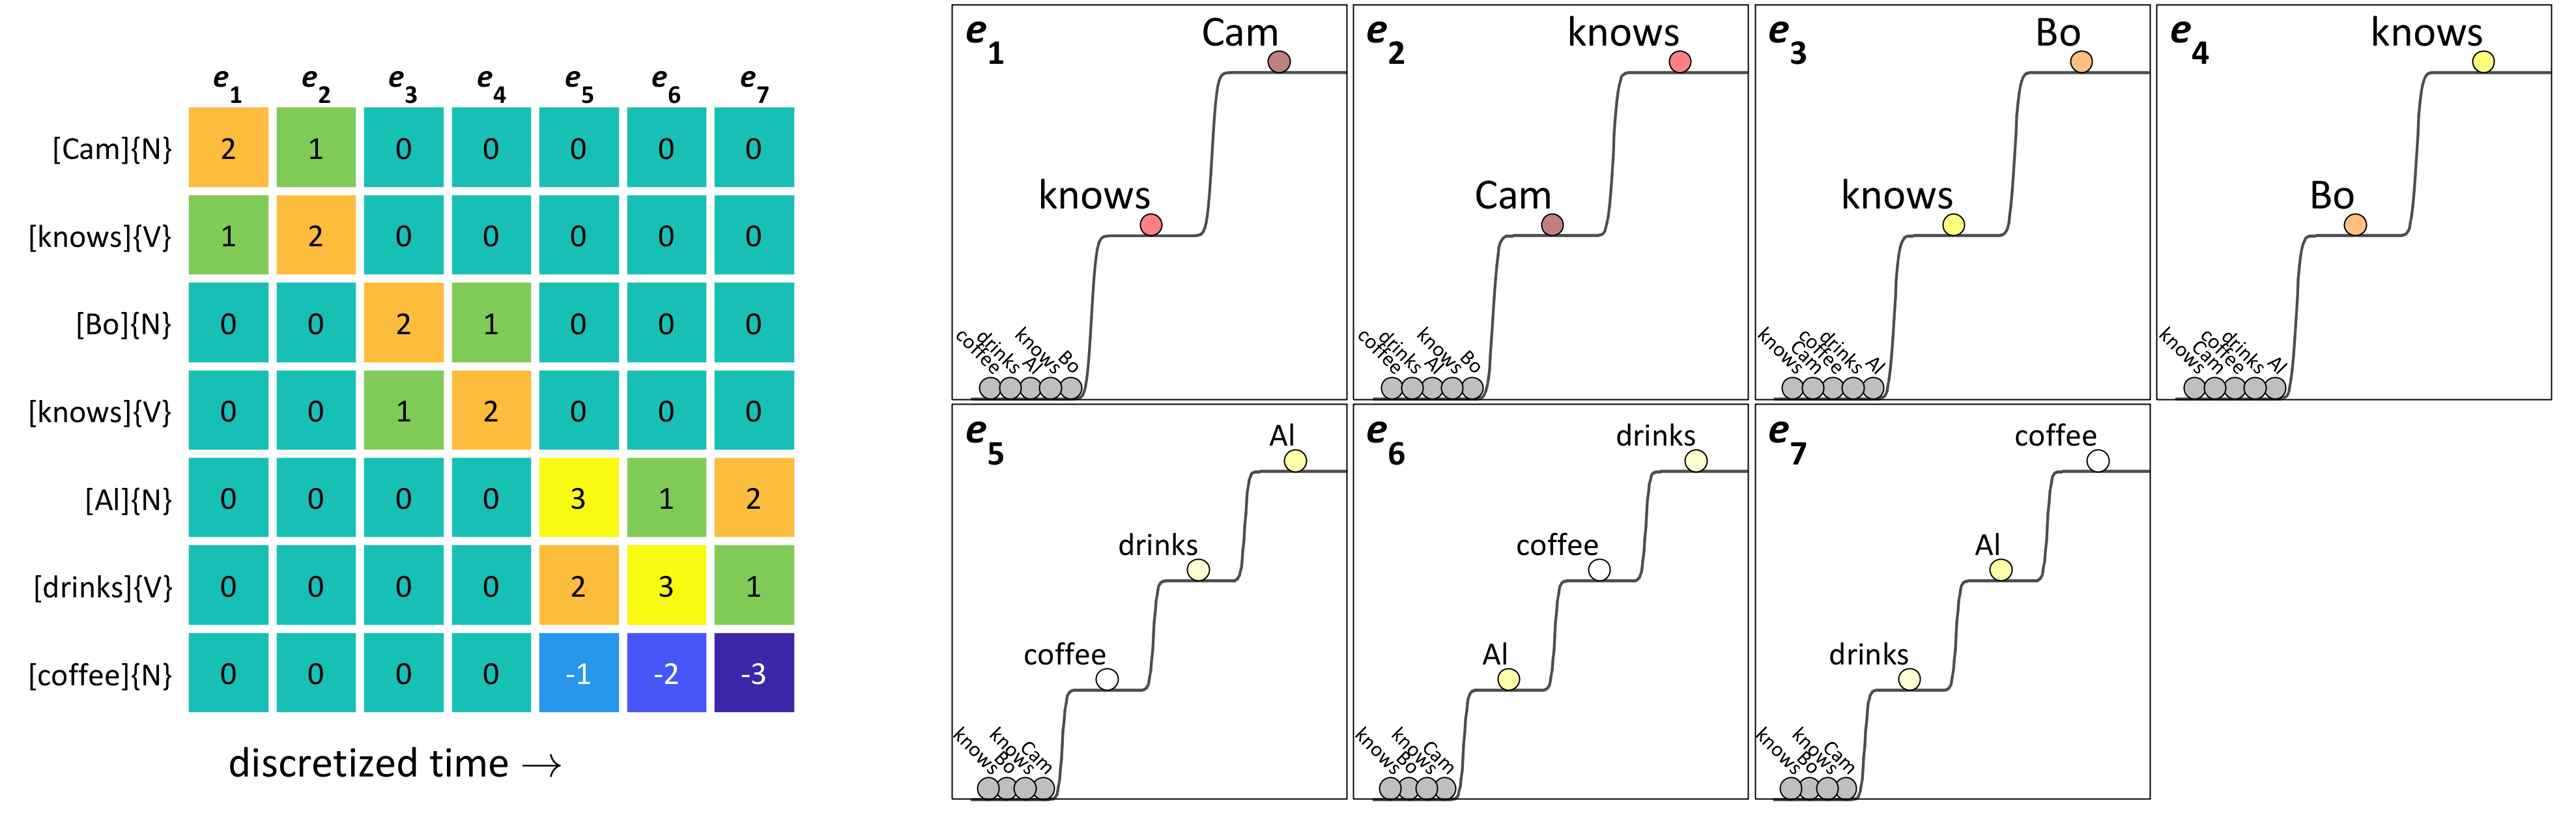
\includegraphics[width=\textwidth]{figures/Tilsen-img112.png}
\caption{Recursion as a trajectory which goes near to a location in state space that was previously visited.}
\label{fig:5:8}
\end{figure}
 

  To distinguish the conventionally recursive utterance from one which would be considered non-recursive, we compare the state vector sequence in {\figref{fig:5:8}} to the one in {\figref{fig:5:9}} for the utterance \textit{Cam knows something. Bo knows something}. In both utterances, the state trajectory returns to nearby locations: $(e1) \approx\allowbreak (e5)$, and (e2)\,${\approx}$\,(e6). The key difference from the conventionally recursive pattern is that intervening between these states is (e4), where no systems are at \isi{selection level}. The state (e4) can be viewed as a relatively large discontinuity in the \isi{state space} trajectory, which disqualifies the similarities (e1)\,${\approx}$\,(e5) and (e2)\,${\approx}$\,(e6) as examples of \isi{recursion}.

  
\begin{figure}
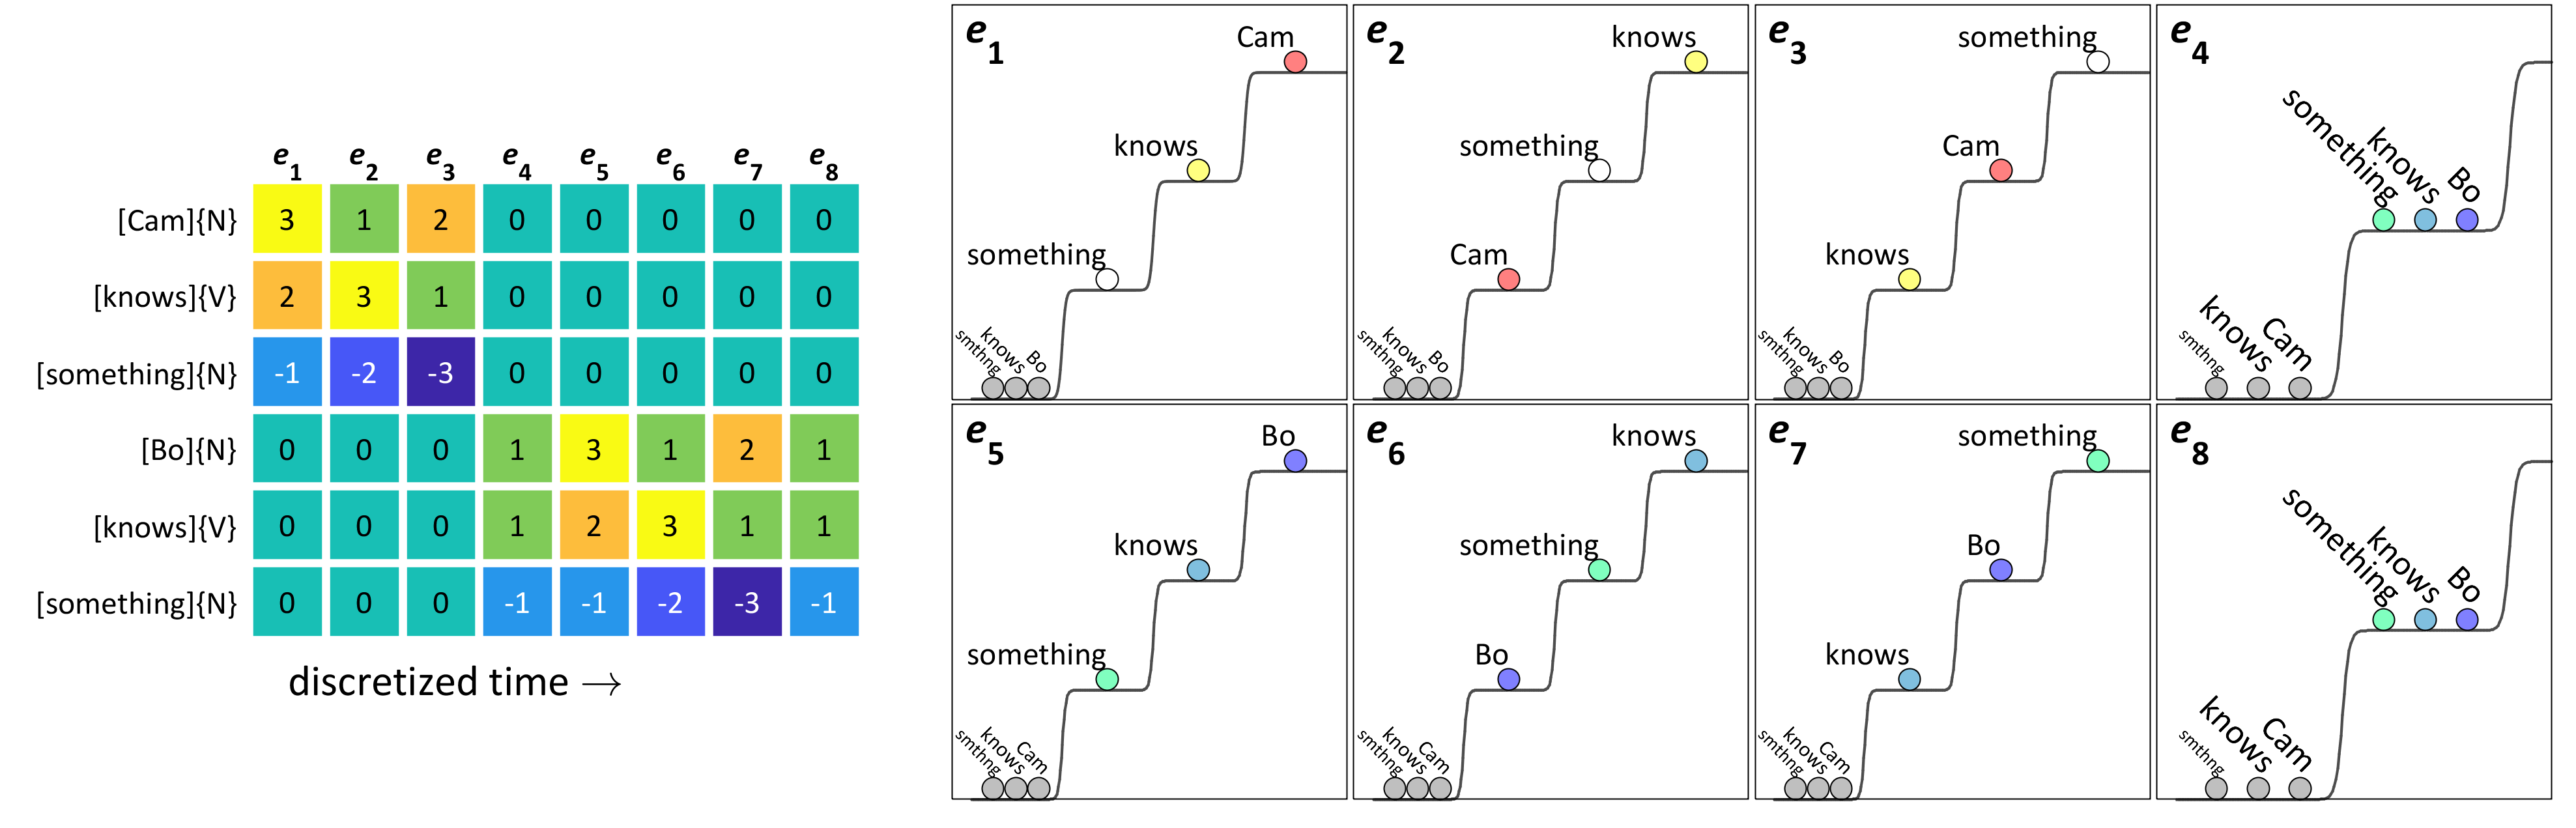
\includegraphics[width=\textwidth]{figures/Tilsen-img113.png}
\caption{Trajectories are not considered recursive when they exhibit a large discontinuity before returning to a previously visited location.}
\label{fig:5:9}
\end{figure}
 

  The criterion for disqualifying similarity between temporally disjoint states as an example of \isi{recursion} is arbitrary: we generally impose the constraint that the disjoint states must be connected by a trajectory in which some s-sys\-tem is always selected. In other words, we assume that between the similar states, no reorganization occurs which fails to promote some s-sys\-tem to \isi{selection level}. Hence if a \isi{speaker} utters \textit{Bo knows}, and then the \isi{speaker} takes a nap, and then utters \textit{Al drinks coffee}, we do not pursue a recursive analysis. 

  The arbitrariness of what we categorize as \isi{recursion} follows not only from our criteria for what sorts of states can intervene between the similar states, but also from the metric of similarity. In the conventionally recursive example in {\figref{fig:5:8}} the (e1) and (e3) states (\textit{Cam knows} and \textit{Bo knows}) are more similar to one another than (e5) (\textit{Al drinks coffee}) is to either (e1) or (e3). This is a consequence of the fact that \{V\}[drinks] has a \{−N\} object. But there are no non-arbitrary criteria for stipulating that (e5) is similar enough to (e3) for the sequence to be considered recursive.

  Furthermore, we must impose an arbitrary criterion for the minimal temporal distance between the similar states. Consider the list utterance \textit{Al drinks coffee, tea, pop, whisky, beer, cider}. We might hesitate to consider lists as examples of \isi{recursion}, even though from a generative perspective, lists are just as recursive as embedded clauses (i.e. \textsc{Merge} builds them). As shown in {\figref{fig:5:10}}, states (e3) through (e8) are all quite similar: there is one highly excited \{−N\} system and a highly excited \{+N\} and \{V\} system.

  
\begin{figure}
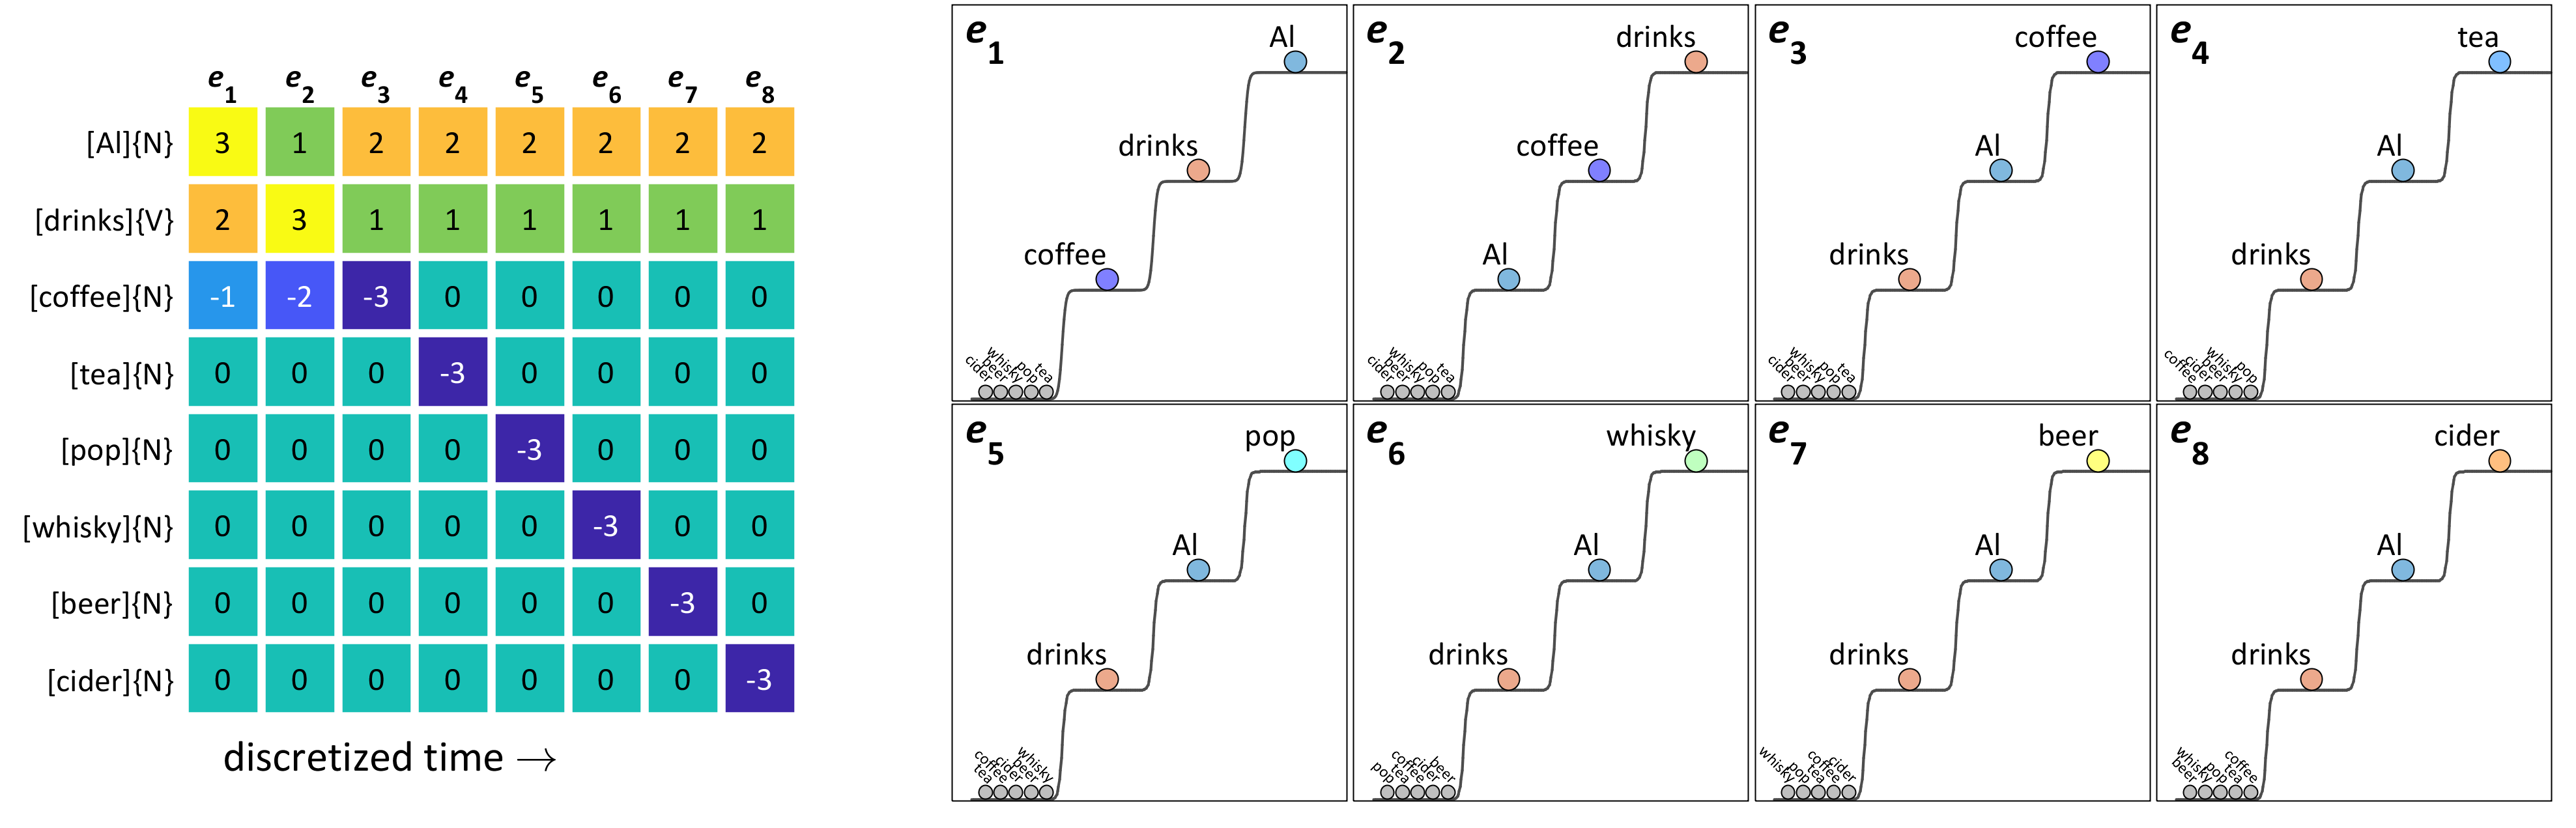
\includegraphics[width=\textwidth]{figures/Tilsen-img114.png}
\caption{Trajectories that stay in the same location are considered less interesting examples of recursion.}
\label{fig:5:10}
\end{figure}
 

  Why do we feel that lists are substandard examples of \isi{recursion}? We seem to prefer for there to be some intervening state(s) between the states which are similar. This reinforces the point that there is no non-arbitrary way of defining \isi{recursion}, because \isi{recursion} is simply the circumstance in which a state is similar to a previous one. The “previous” and “similar” qualifiers require arbitrary temporal and spatial criteria. 

  The o/el way of thinking changes the sort of questions we can ask about \isi{recursion}. Instead of being interested in “\isi{embedding depth}” and spatial patterns of connected objects structures, we can ask about the e-operations that intervene between states, the dimensions in which we construct an understanding of the states, and the proximity of the locations of those states in our analytically constructed spaces.

\subsection{Reiterative simulation}

Here we introduce a new sense of \isi{recursion}, \textit{\isi{reiterative} simulation}, which is useful for various analyses of syntactic phenomena in subsequent chapters. Recall that thresholding mechanisms in production allow for a cs-simulation regime in which s-gates are open but m-gates are closed. Because this regime does not engage gm-selection, we do not experience the sensory consequences of selection in the same way that we do for gm-simulation (i.e. \isi{subvocal rehearsal}). Thus we are not necessarily “aware” of cs-simulation in the same way that we are “aware” of gm-simulation.

  What patterns of reorganization might occur in cs-simulation? One possible hypothesis is that only exactly the same e-reorganizations occur as those we hypothesize for gm-simulation/execution trajectories. An alternative we pursue here is that cs-simulation often enters a \isi{reiterative} regime, in which a trajectory of e/ϕ-con\-fig\-u\-ra\-tions is reiterated an arbitrary number of times, giving rise to a periodic state trajectory on supra-clausal scales. This sort of trajectory is more practical in cs-simulation because reorganization operations need not depend on gm-selection feedback.

  To see why \isi{reiterative simulation} is useful, let's consider two utterances: \textit{Bo knows Al drinks coffee} and \textit{Al drinks coffee, Bo knows}. From the perspective of a producer or \isi{interpreter}, the state trajectories of these utterances are very similar, except that the two ϕ-con\-fig\-u\-ra\-tions are executed/evoked in different orders. Let's imagine that a producer, prior to execution, engages a \isi{reiterative simulation}. The \isi{reiterative trajectory} we envision is shown in {\figref{fig:5:11}}. (To reduce visual clutter e-levels within clauses are not differentiated in the e-potentials.) The \isi{reiterative simulation} alternates between subtrajectories in which {\textbar}Bo knows{\textbar} and {\textbar}Al drinks coffee{\textbar} configurations are excited. This gives rise to a periodic trajectory with two ϕ-epochs,  labeled (e) and (e′). In general, each ϕ-epoch contains one or more e-epochs.

  
\begin{figure}
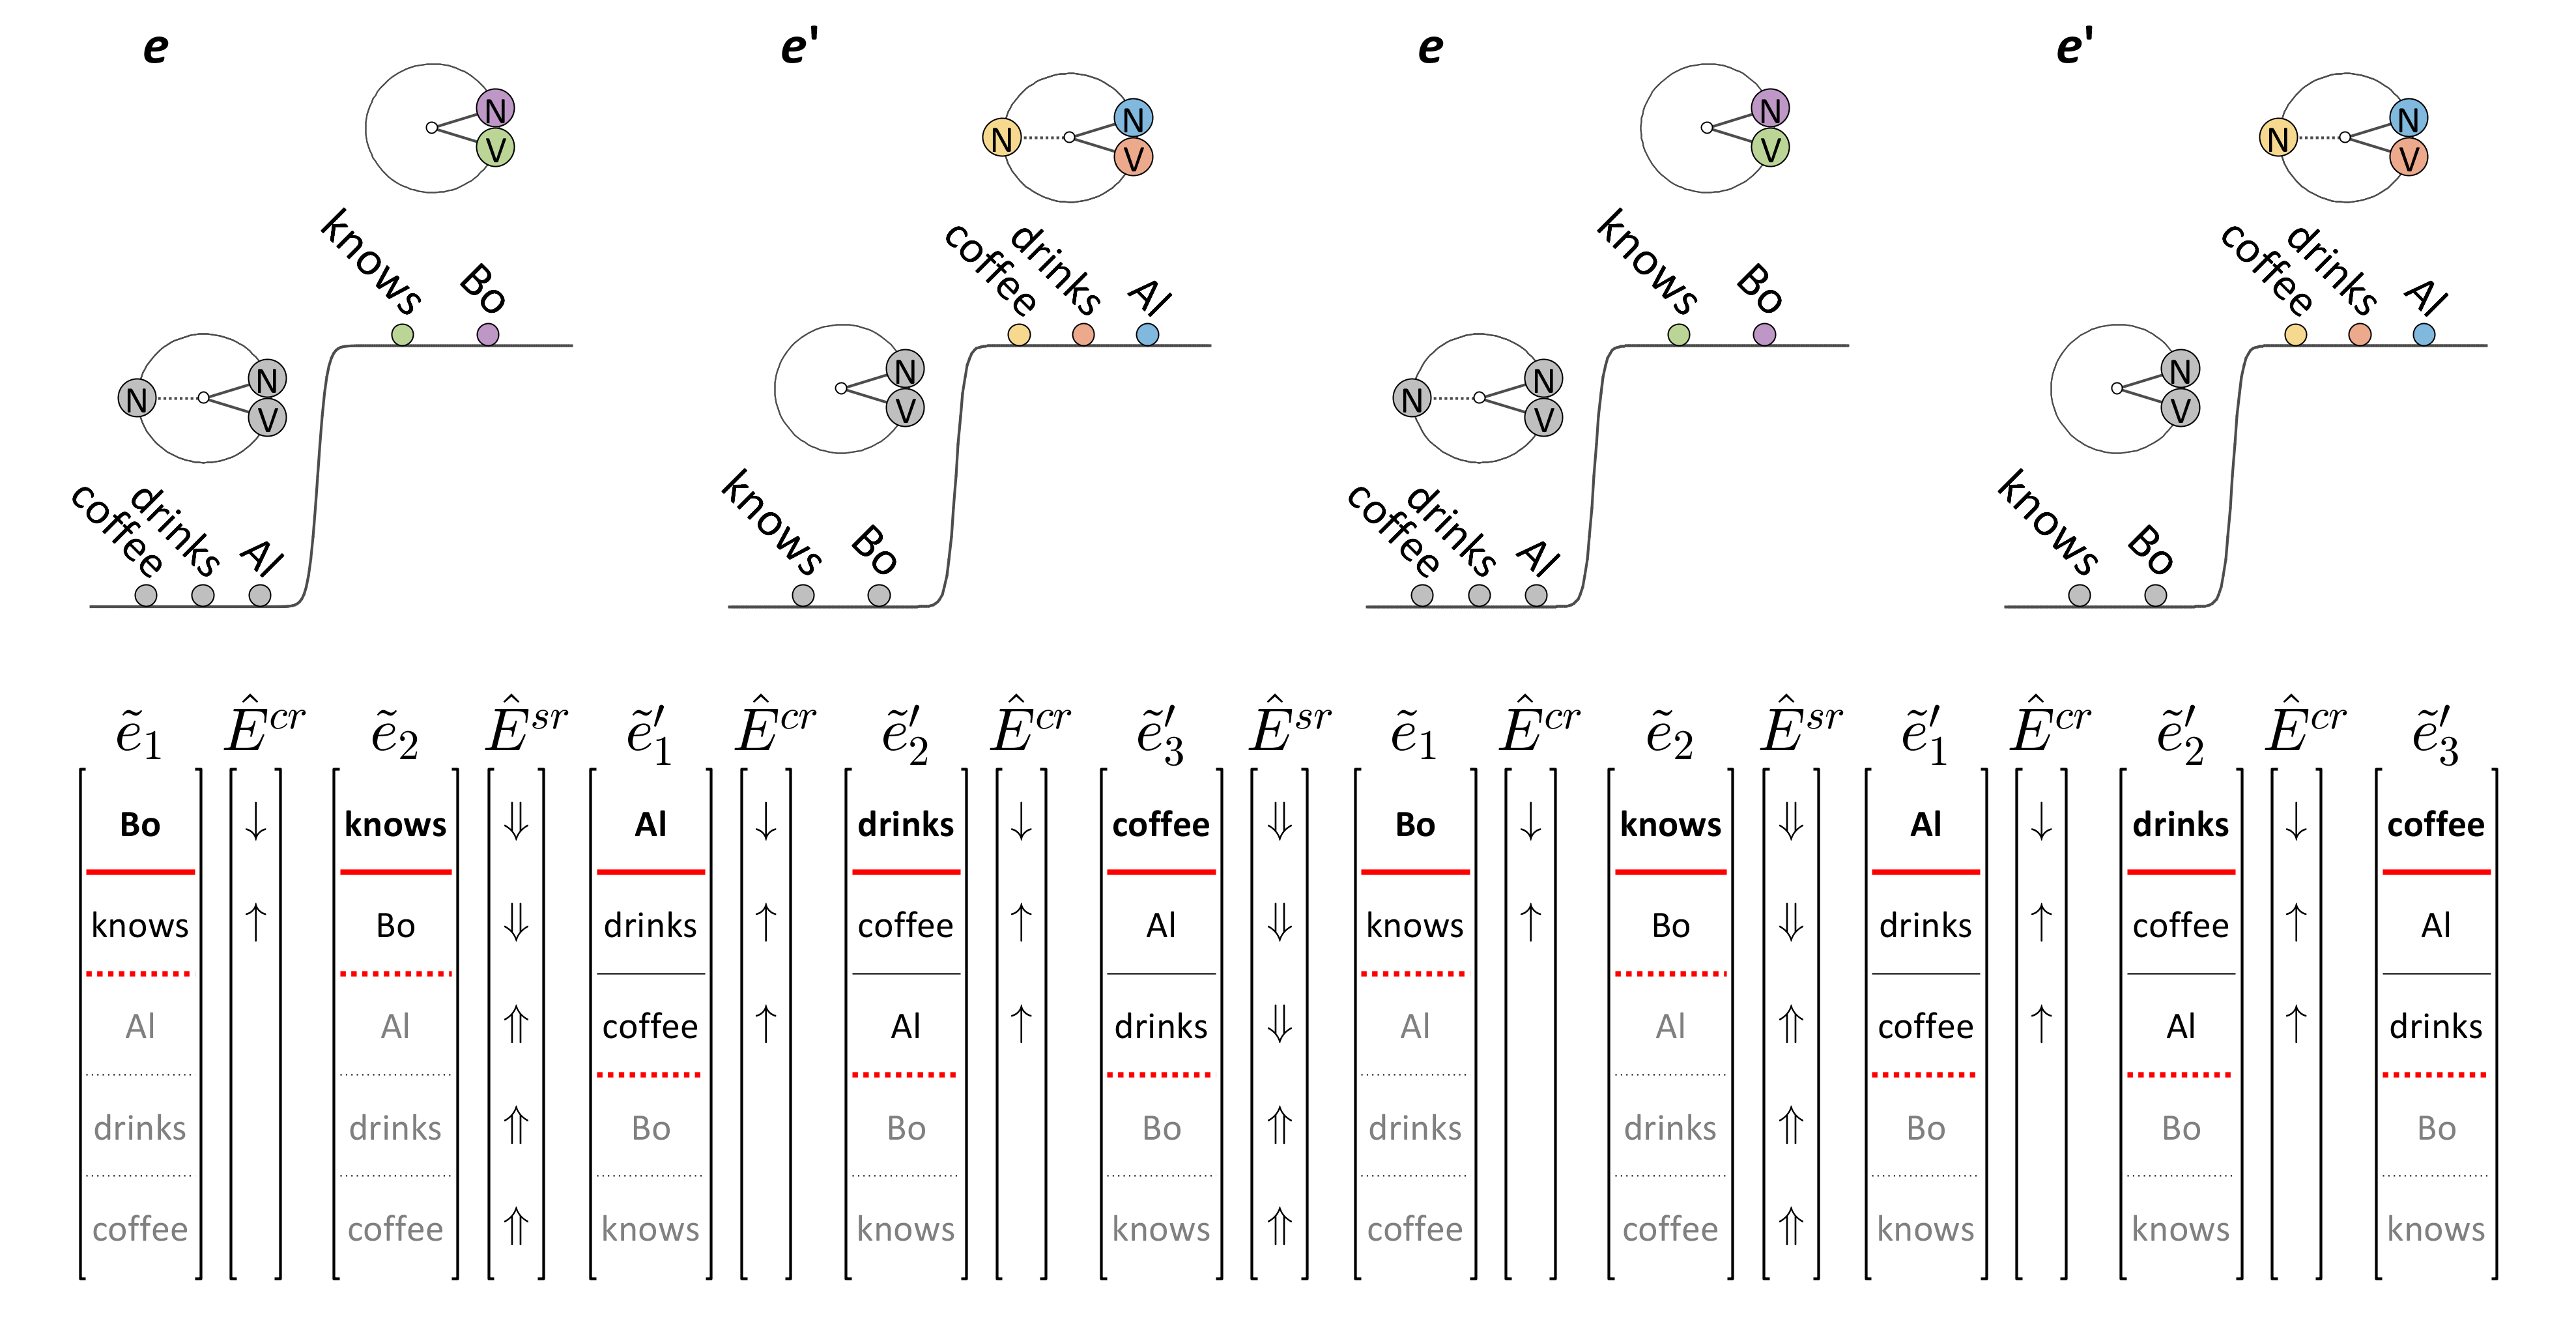
\includegraphics[width=\textwidth]{figures/Tilsen-img115.png}
\caption{In a reiterative simulation, there is no global notion of precedence of ϕ-con\-fig\-u\-ra\-tions.}
\label{fig:5:11}
\end{figure}
 

  An important consequence of having a periodic trajectory is that any global notion of \isi{precedence} becomes arbitrary. As such, neither ϕ-epoch precedes the other: {\textbar}Bo knows{\textbar} and {\textbar}Al drinks coffee{\textbar} configurations are \isi{unordered}; a discrete time translation symmetry is created. We might also imagine that an \isi{interpreter} trajectory can evolve to be \isi{reiterative}, again rendering any global notion of \isi{precedence} arbitrary. In a sense, the echoes of production which interpreters experience restore a symmetry that was broken in overt production. 

  Put somewhat differently, the loss of \isi{precedence} information is a key condition for invariance of meaning experiences, on both e-epoch and ϕ-epoch scales. For a single e-epoch, a \isi{relational meaning} experience is a stable periodic trajectory of cs-sys\-tems. The discrete translational symmetry of the trajectory in θ subspace makes it impossible to decide which member of a set of cs-sys\-tems “comes first” -- \isi{precedence} information is lost. Likewise, for a ϕ-epoch, a \isi{reiteration} of epochs creates the discrete translational symmetry which destroys \isi{precedence} information: it is not possible to say which ϕ-con\-fig\-u\-ra\-tion precedes the other. The loss of \isi{precedence} information is fundamental to invariance. 

  Reiterative simulation also provides a mechanism for understanding sources of variation in order of selection during ungated production. Earlier we suggested that \isi{surroundings} forces in the \isi{pre-stable phase} may give rise to variation in initial e-organization. For example, the utterance \textit{Al drinks coffee, Bo knows} might be produced when [Al][drinks][coffee] c-sys\-tems are more highly excited than [Bo][knows] systems. Alternatively, the timing of the transition from a \isi{reiterative} cs-simulative regime to a gm-simulative/executional regime could give rise to variation in production. As shown in {\figref{fig:5:12}}, the order of epochs of \isi{selectional production} in (e1)--(e5) is determined by when the transition to a \isi{selectional regime} occurs in the context of a \isi{reiterative} regime (e, e′).

  
\begin{figure}
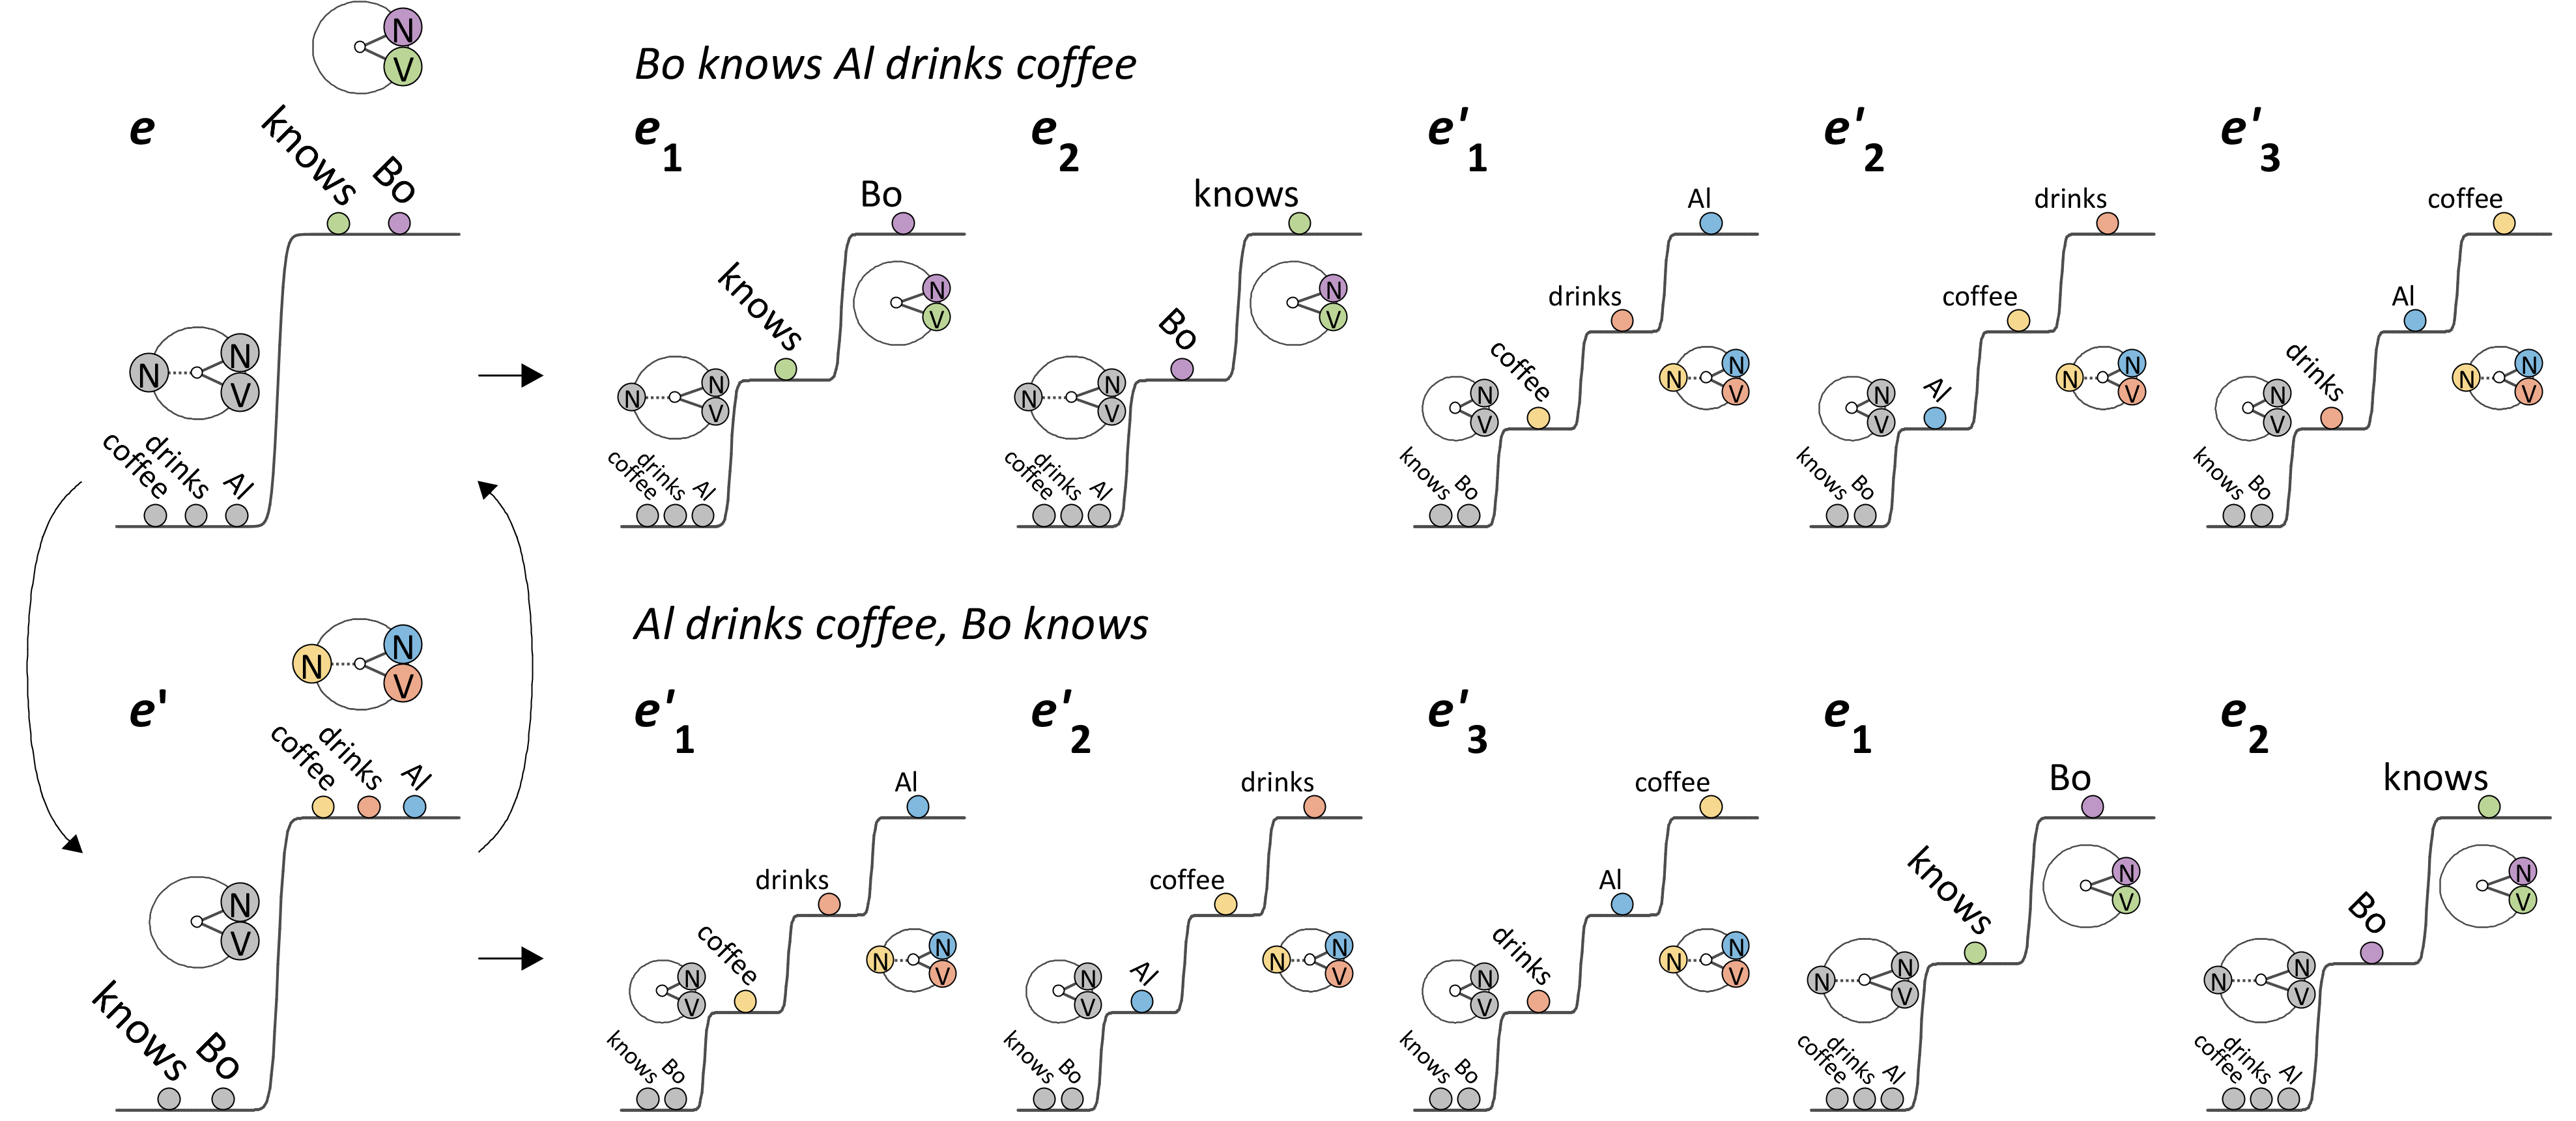
\includegraphics[width=\textwidth]{figures/Tilsen-img116.png}
\caption{Variation in clause order can be generated from when a producer transitions to an executional regime, in the cycle of a reiterative simulation.}
\label{fig:5:12}
\end{figure}
 

  Another potential consequence of \isi{reiterative simulation} could be to stabilize simultaneous excitation of ϕ-con\-fig\-u\-ra\-tions. As depicted in {\figref{fig:5:12}}, this could be accomplished by promoting frequency locking between systems, which would diminish the decohering effects of \isi{interference}. Thus we speculate that \isi{reiterative simulation} could allow for simultaneous excitation of configurations which might otherwise be unstable and which would need to be selectively re-or\-ga\-nized.

  
\begin{figure}
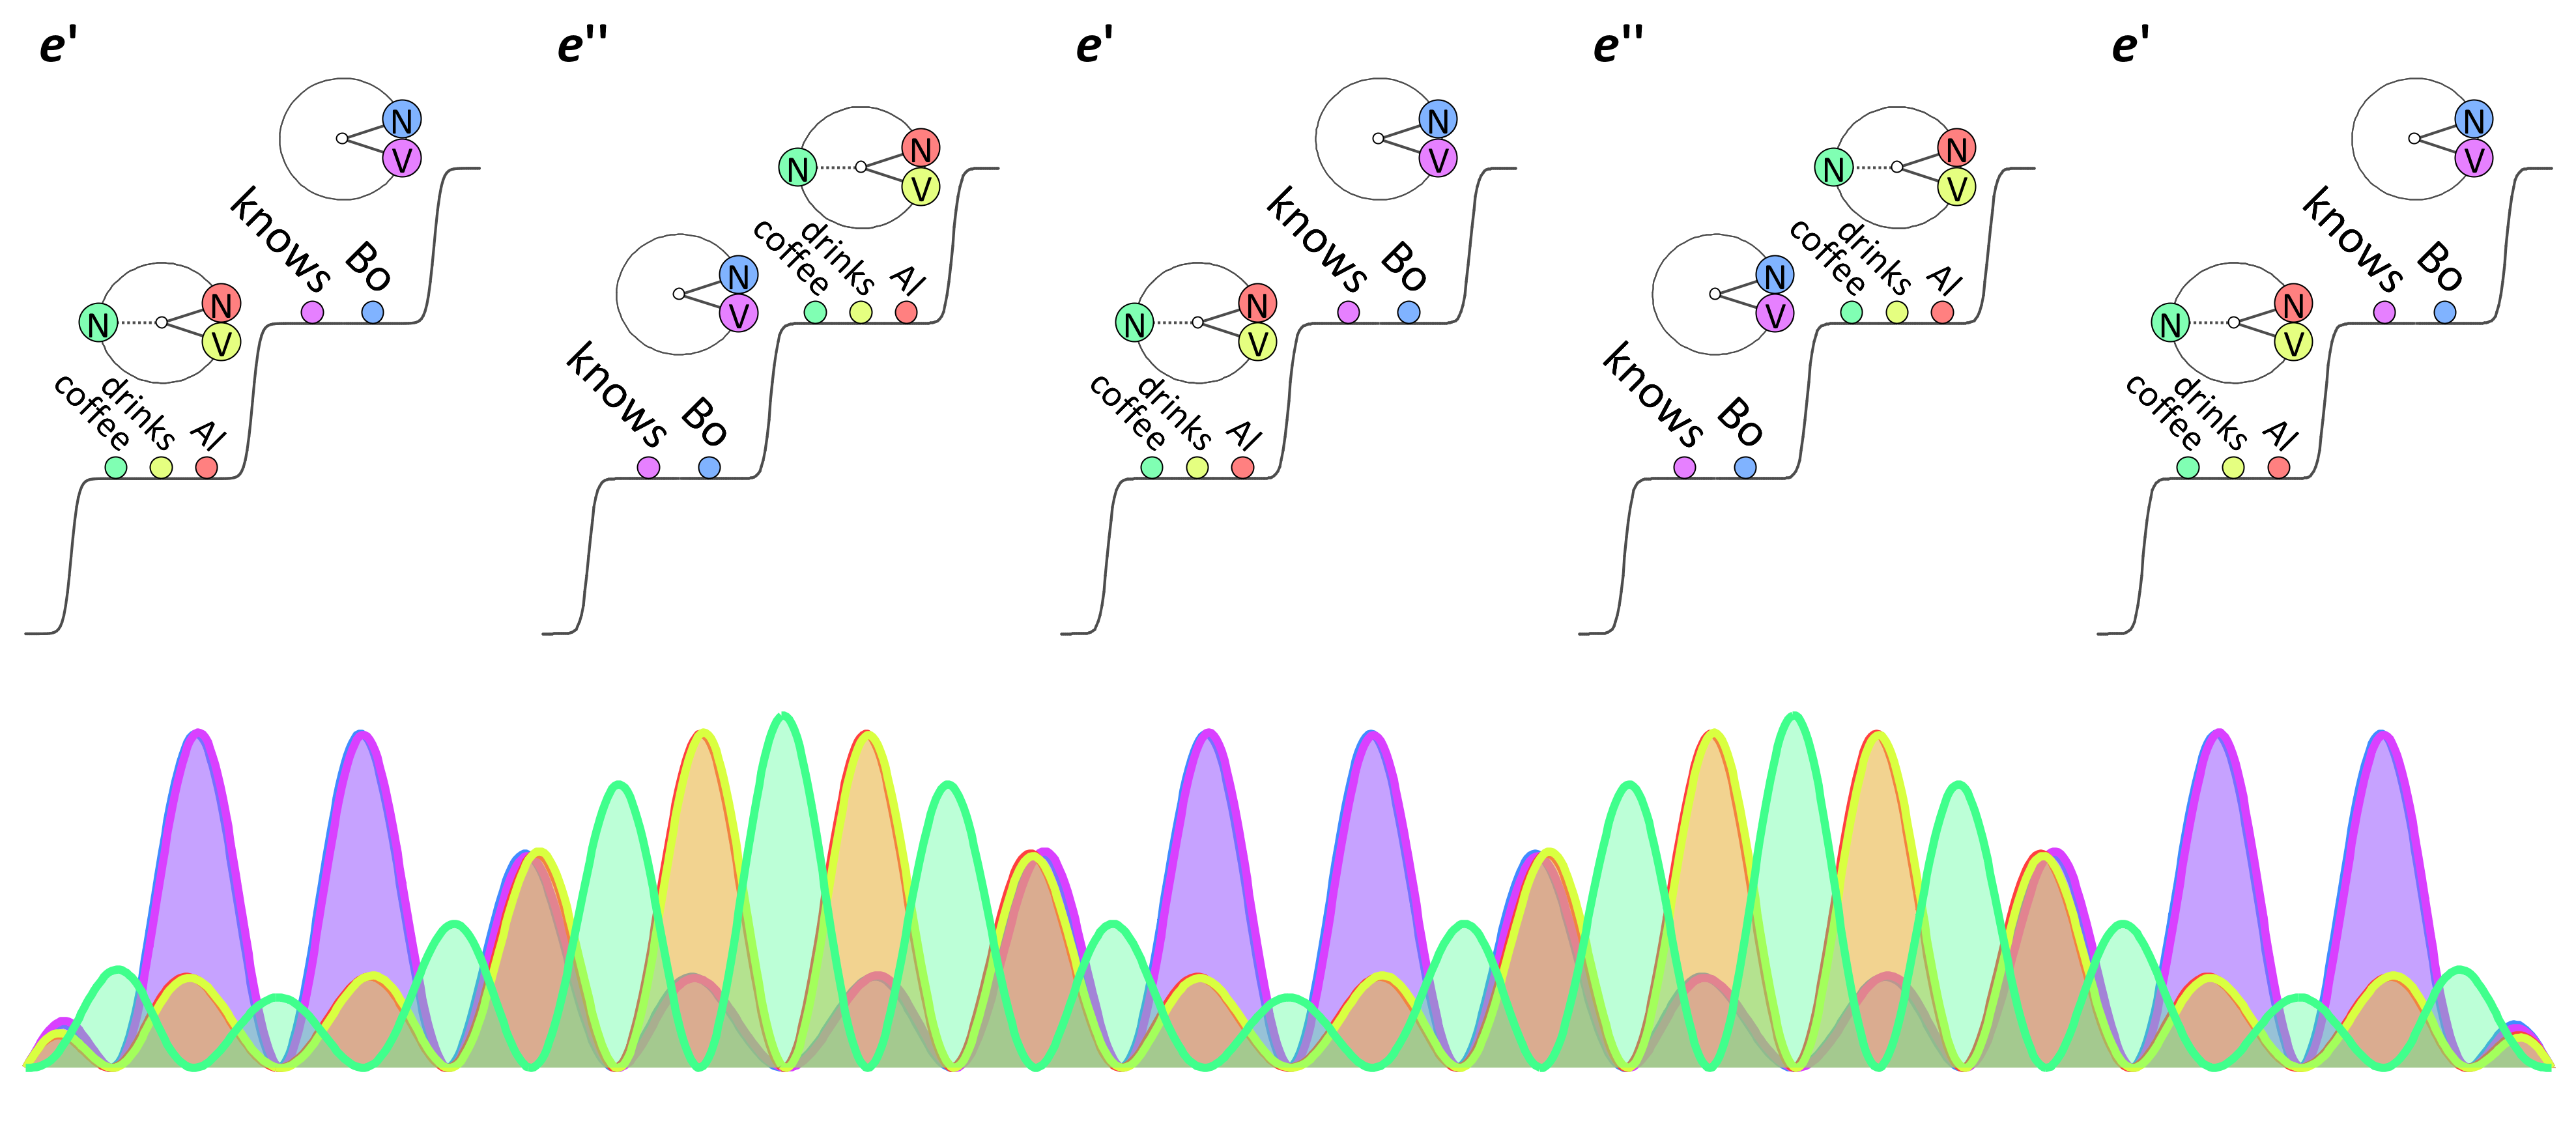
\includegraphics[width=\textwidth]{figures/Tilsen-img117.png}
\caption{Reiterative simulation may help stabilize the excitation of multiple ϕ-con\-fig\-u\-ra\-tions by promoting frequency locking between configurations, thereby diminishing interference.}
\label{fig:5:13}
\end{figure}
 

  Reiterative simulation is a form of “\isi{recursion}” because stable ϕ/e-con\-fig\-u\-ra\-tions \textit{recur}, i.e. the \isi{state space} trajectory returns to previous states. Unlike conventional \isi{recursion}, which applies only to s-sys\-tems and requires arbitrary similarity and time constraints, the \isi{reiterative simulation} variety of \isi{recursion} can be defined with both c- and s-sys\-tem states and has easy-to-motivate constraints. Reiterative cs-simulation may occur pervasively, and yet because such trajectories are m-gated, we may not be very aware of them. 

\subsection{Embedding vs. reorganization}

So-called “embedded” structures are the parade examples of conventional \isi{recursion}. How does the o/el model conceptualize these, if not with containment and connection? First, we emphasize that there is no notion of embedding without the \isi{object metaphor} and connection/\isi{containment blend}. This is clear when we reflect on why some patterns are better or worse examples of \isi{recursion}. Tail \isi{recursion}, as shown in {\figref{fig:5:14}}(A), can evoke a schema of containers inside containers. Tail \isi{recursion} is considered somewhat less worthy as an example of \isi{recursion} because it is easy to replace the nested containers with a sequence of adjacent ones (A′). Center embedding (B) is a more worthy example of \isi{recursion} because the mirror spatial symmetry of object dependencies maps nicely to nested containers, when the objects are arranged in a line (i.e. \textsc{temporal order is spatial arrangement}). In contrast, scrambling (C) requires \isi{internal merge} (i.e. movement, spatial re-arrangement) and is not consistent with any nested \isi{container schema}.

\begin{table}
\begin{tabularx}{\textwidth}{lQQ}
\lsptoprule
Tail \isi{recursion}: & \textit{Bo knows Al, who drinks coffee} \\
 & \textit{Cam likes Bo, who knows Al, who drinks coffee.}\\
Center embedding: & \textit{Al, who Bo knows, drinks coffee}\\
 & \textit{Al, who Bo, who Cam likes, knows, drinks coffee.}\\
Scrambling: & \textit{Al, Bo, drinks coffee, knows.}\\
 & \textit{Al, Bo, Cam, drinks coffee, knows, thinks.}\\
\lspbottomrule
\end{tabularx}
\caption{Examples of recursive sentences.}\label{tab:5:3}
\end{table}
  
\begin{figure}
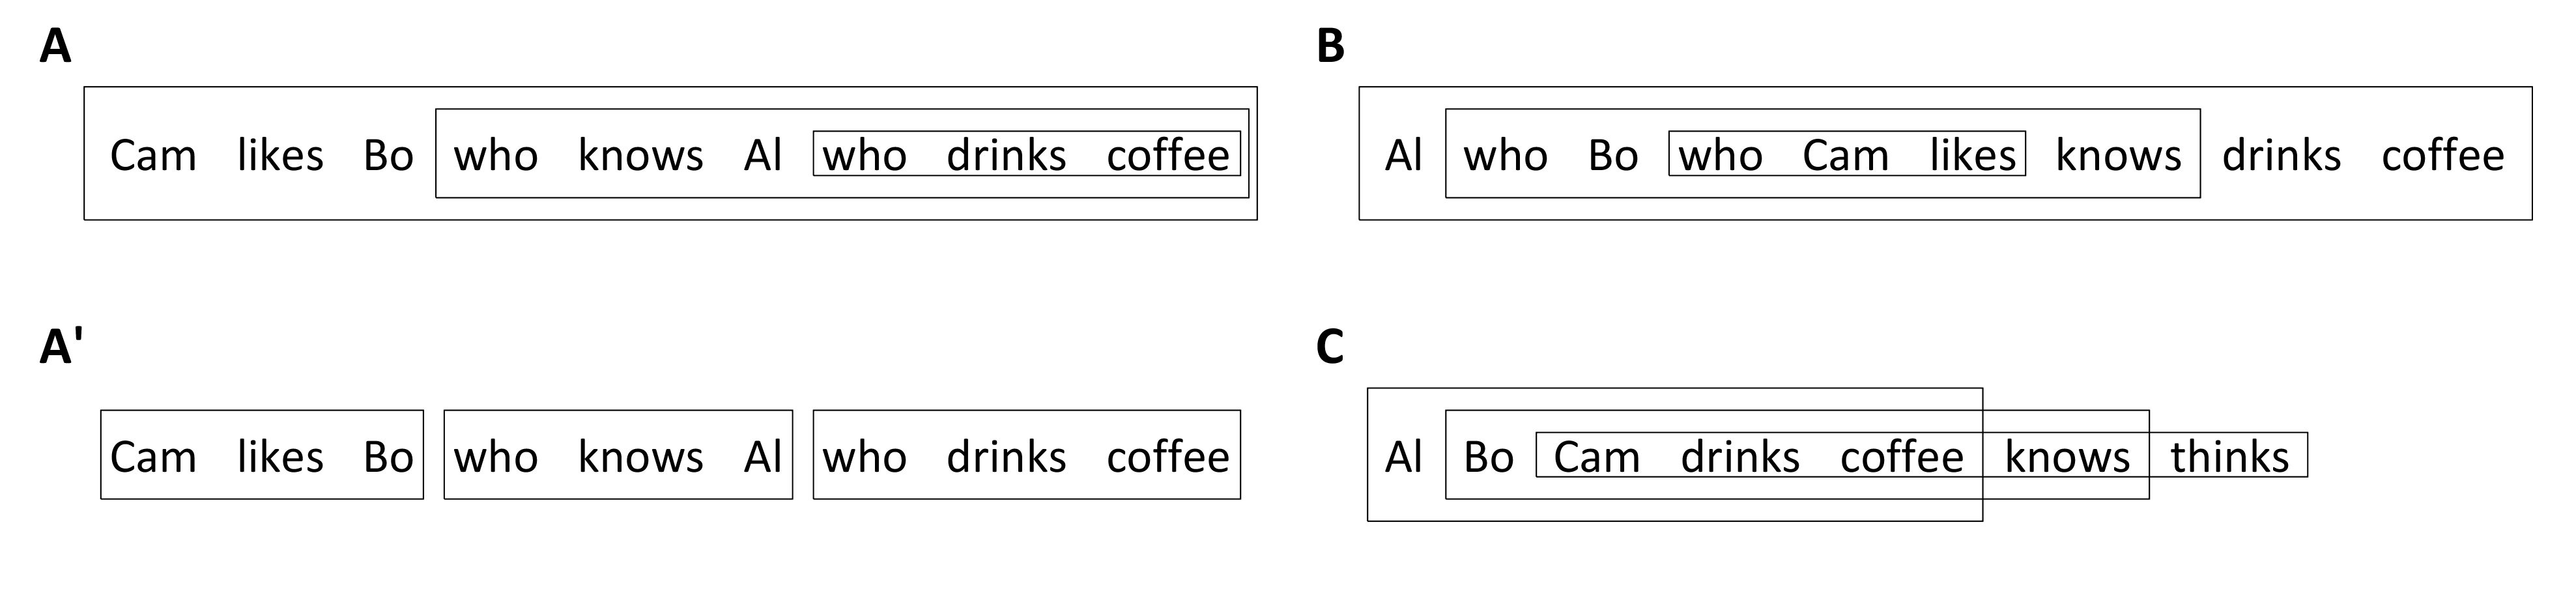
\includegraphics[width=\textwidth]{figures/Tilsen-img118.png}
\caption{Containment schemas for recursive sentences.}
\label{fig:5:14}
\end{figure}
 

  In the o/el framework, patterns such as \isi{tail recursion}, center embedding, and scrambling (shown in {\tabref{tab:5:3}}) result from special reorganization operations that change the relative excitation of systems. If the operations create too much \isi{interference}, the resulting configurations may be unstable. In examining trajectories of “embedded” patterns, we will see that the special reorganizations associated with center embedding and scrambling give rise to more \isi{interference} than \isi{tail recursion}. This explains why center embedding and scrambling are much less common in production and less coherent in interpretation than \isi{tail recursion} (a.k.a. right-branching \isi{recursion}), especially when the number of clauses involved exceeds two \citep{ChristiansenChater1999}. 

  Recall from previous chapters that we have posited several regimes of the e-organization operator. The \isi{stabilizing regime}, which applies within e-epochs, maps e-con\-fig\-u\-ra\-tions to themselves. The canonical \isi{reorganization regime} Ê\textsuperscript{cr} demotes selected systems to the lowest above-ground level and promotes all other excited systems one level. The \isi{selective reorganization} regime Ê\textsuperscript{sr} demotes some systems to ground and promotes some grounded system(s) to excited states. Reiterative simulation results from iterated application of Ê\textsuperscript{cr} and Ê\textsuperscript{sr}. We also posited an \isi{initial organization operator} Ê\textsuperscript{io} to map from a pre-stable state to a stable, discrete configuration.

  The operators Ê\textsuperscript{cr} and Ê\textsuperscript{sr} can be decomposed into more basic, element-wise promotion and demotion operators, ↑ and ↓. Generally, any reorganization operation can be characterized based on whether the systems in its domain (inputs) and range (outputs) are ground-level, excited, or selected systems. This results in 3 distinct domain and range patterns, a total of 9 possibilities. The {\tabref{tab:5:4}} summarizes the classification.

\begin{table}
\small
\begin{tabularx}{\textwidth}{c c@{~}c@{~}c c@{~}c@{~}c X}
\lsptoprule
& \multicolumn{3}{c}{input} & \multicolumn{3}{c}{output} & \\
& ground & excited & selected & ground & excited & selected & \\
\midrule
 $\Uparrow $ & + & \textminus & \textminus & \textminus & + & + & \isi{ungrounding promotion}\\
&  &  &  & \textminus & + & \textminus & \\
\hline
 1 & + & \textminus & \textminus & + & \textminus & \textminus & identity\\
 \hline
 ↑ & \textminus & + & \textminus & \textminus & + & + & canonical promotion\\
&  &  &  & \textminus & + & \textminus & \\
\hline
 $\Downarrow $ & \textminus & + & \textminus & + & \textminus & \textminus & \isi{grounding demotion}\\
& \textminus & + & + &  &  &  & \\
\hline
 1 & \textminus & + & + & \textminus & + & + & identity\\
 \hline
 ↓ & \textminus & + & + & \textminus & + & \textminus & canonical demotion\\
\lspbottomrule
\end{tabularx}
\caption{Classification of reorganization operations.}\label{tab:5:4}
\end{table}

  The \isi{ungrounding promotion} operator $\Uparrow $ promotes a ground-level system to an excited (possibly selected) level, while the canonical promotion operator ↑ promotes an already excited system. There may be analyses for which it is useful to distinguish between promotion to non-selected excitation and selection. The \isi{grounding demotion} operator $\Downarrow $ demotes an excited (often selected) system to ground-level, while the  canonical demotion operator ↓ demotes a selected system to an above-ground (typically the lowest) level. An arbitrary reorganization vector Ê consists of these basic operations and acts element-wise on an e-organization vector  $\widetilde{{e}}$, which is obtained by permuting the system state vector such that the dimensions are ordered according to system e-levels.

  Tail \isi{recursion}, center embedding, and scrambling trajectories can be generated through appropriate choices for the components of Ê. For instance, compare the trajectories of examples of \isi{tail recursion} (A) and center embedding (B) in {\figref{fig:5:15}}. Both examples have three clauses, but the \isi{tail recursion} requires just two selective reorganizations, while the center embedding requires four. The selective reorganizations of the \isi{tail recursion} promote and demote clause-like ϕ-con\-fig\-u\-ra\-tions, while the promotions and demotions of the selective reorganizations in center embedding apply to sub-clausal sets of cs-sys\-tems. Furthermore, the \isi{tail recursion} maintains at most four systems in an \isi{excited state}, and none of these interfere; in contrast, the center embedding maintains up to six cs-sys\-tems above ground. Several of those systems interfere, namely [Cam], [Bo], and [Al]. Promotion of one of these systems from ground, without demotion of potentially interfering systems, can destabilize the system. Perhaps what is most problematic is that in epochs (e1)--(e3) of the center embedding, there are \{N\} systems which are not ϕ-coupled to any \{V\}.

  
\begin{figure}
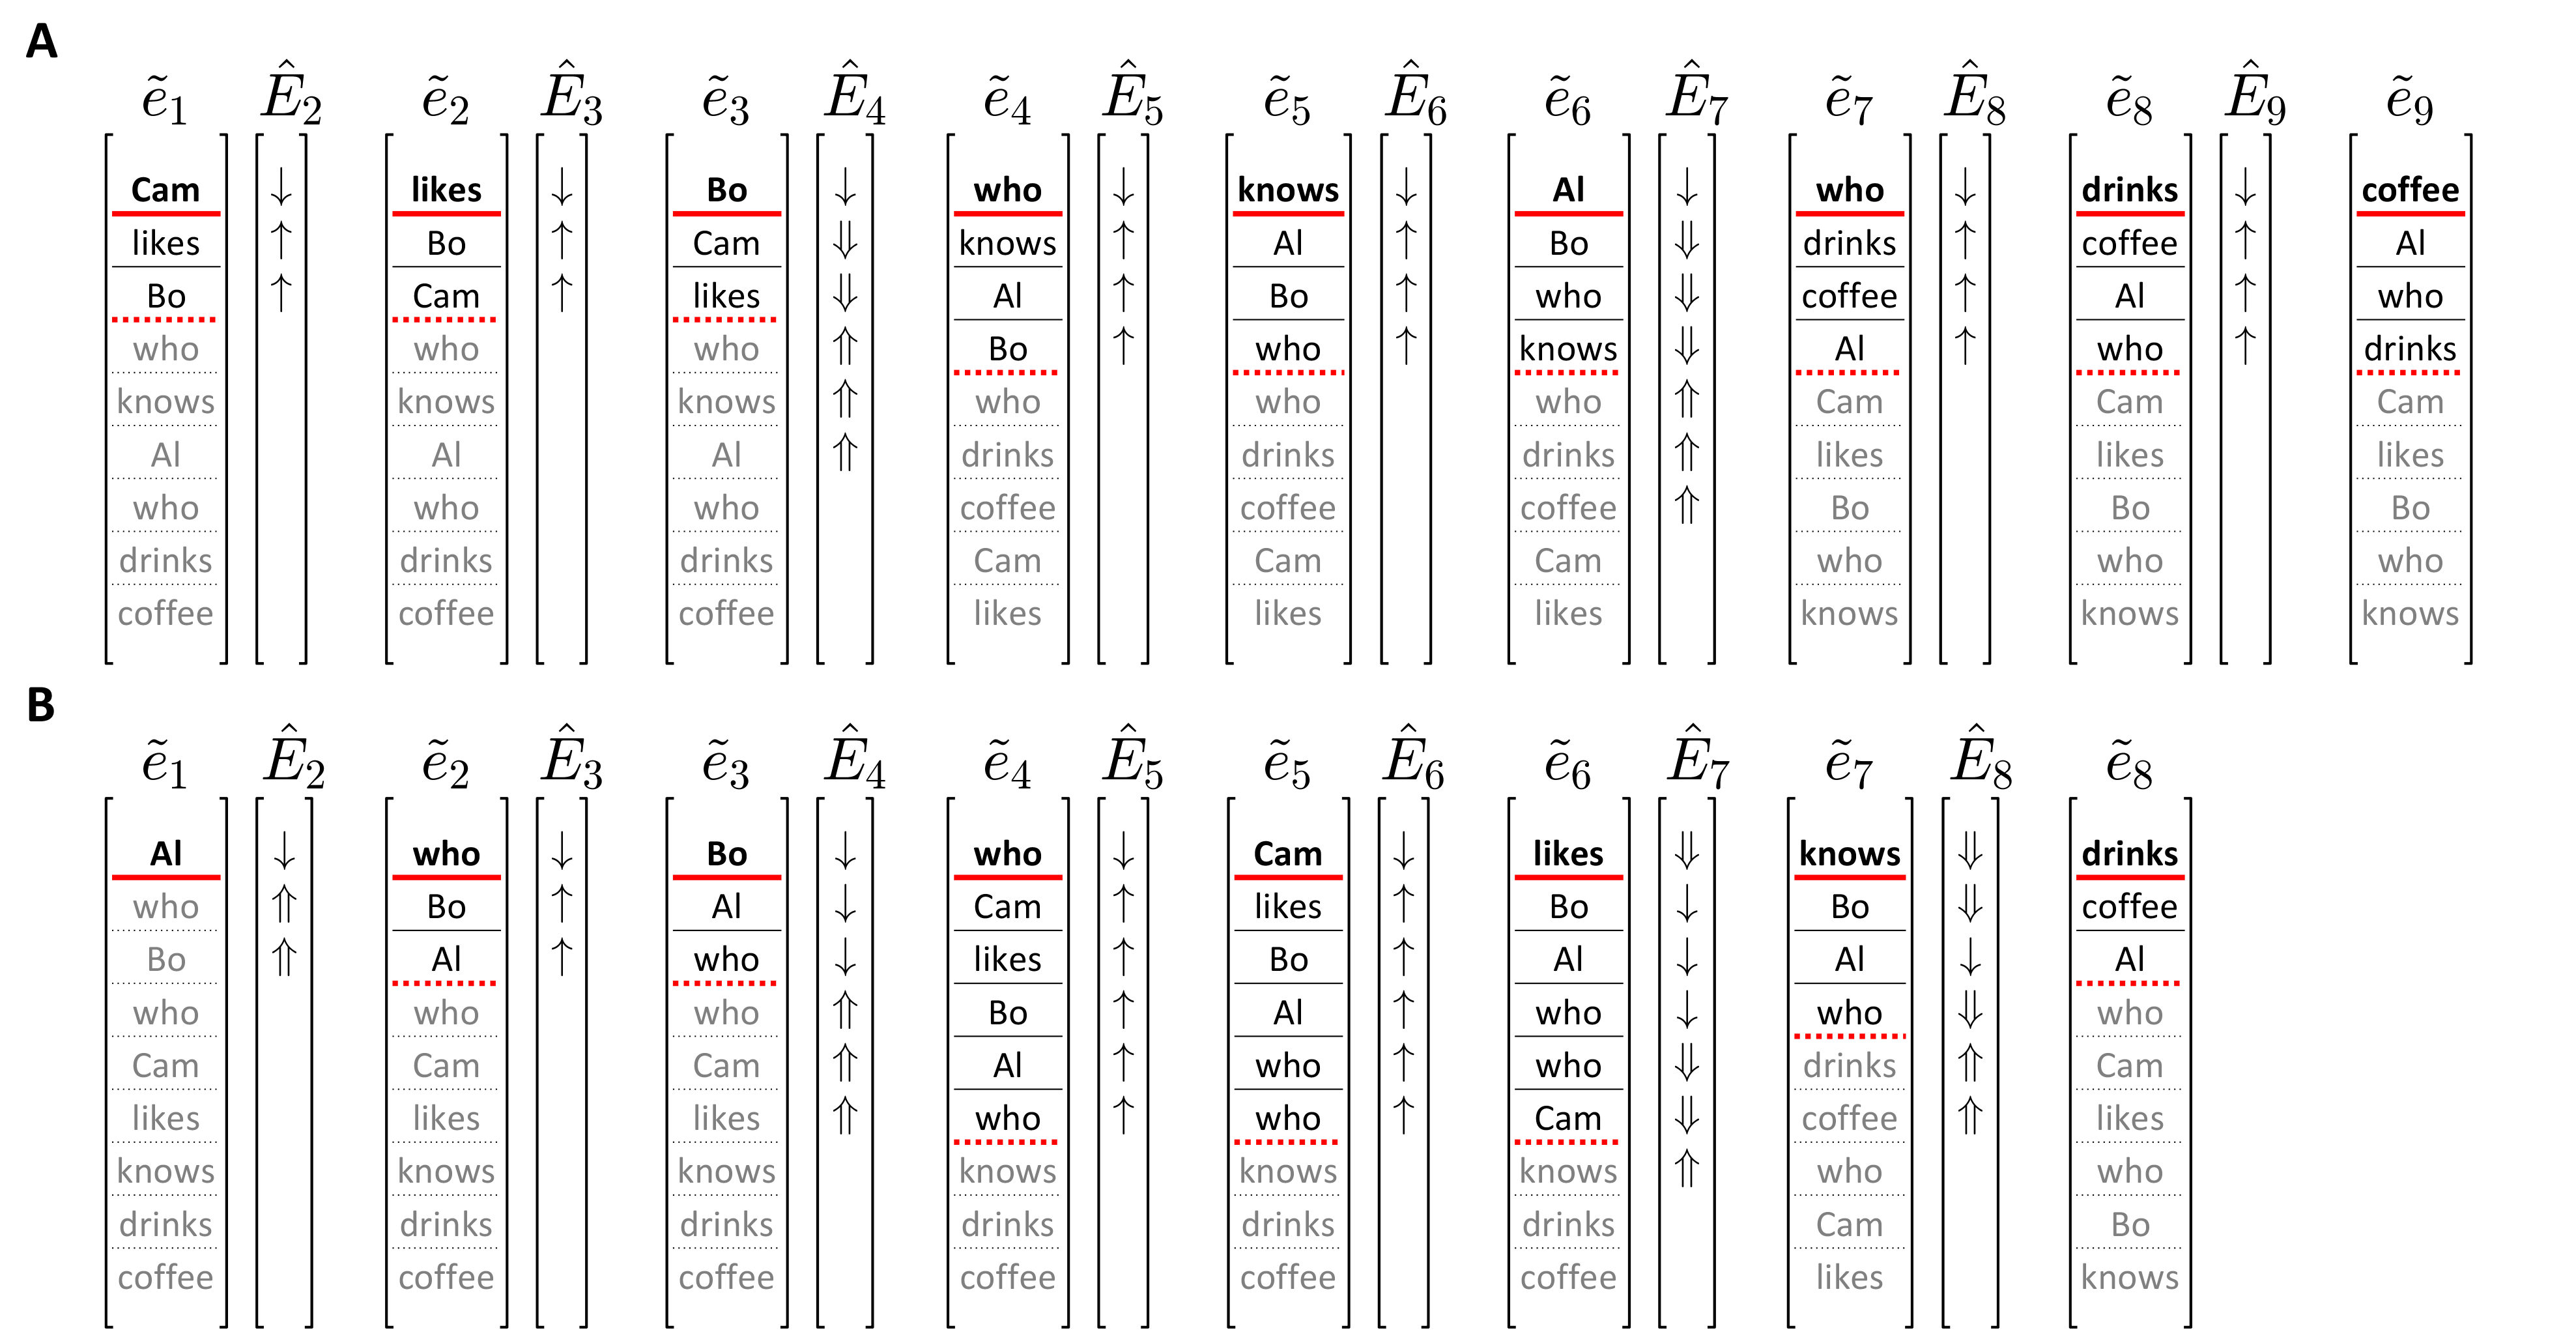
\includegraphics[width=\textwidth]{figures/Tilsen-img119.png}
\caption{Example trajectories for tail recursion and center embedding.}
\label{fig:5:15}
\end{figure}
 
   The analyses above are not the only possible ones, and we can imagine viable alternatives. For example, [drinks]\{V\} and [coffee]\{−N\} might have been excited in (e1) and demoted to ground in (e2), or even remain above ground, creating further \isi{interference} with [likes] and [knows] in subsequent epochs. There are numerous sensible possibilities for how a scrambling trajectory might arise. The relevant systems might be initially grounded and selectively promoted from ground during selective production; alternatively, the systems might be initially organized such that a single clause is excited, and subsequently selective reorganizations generate the scrambled trajectory. Motivating any particular analysis of Ê operations in scrambling is an open challenge. Yet because center embedding and scrambling rarely involve more than two clauses, we should not overemphasize the importance of such examples.

  The applications of reorganization operations employed in the above analyses raise the question of what constraints there are on Ê. Although we do not systematically pursue this question in great detail, one clear generalization is that promotion and demotion co-occur and often affect similar subsystems in a given transition. This makes sense given that we view e-operations as the consequence of e-coupling forces, and that e-coupling forces are expected to be stronger between more similar systems. We have also imposed a number of analytic choices which warrant further scrutiny. For instance, we have assumed that once the selective regime of production begins, no epochs without a selected system occur. This assumption could be violated, and one can imagine decomposing each Ê into an ordered sequence of operations on individual systems. The order of these operations could matter.

  Clearly a principled theory of constraints on reorganization operations is desirable, and in the absence of such a theory the reorganization mechanism seems overly powerful. For the time being, we can decide to accept this because we have not mistakenly imposed structure where none is present. Whereas the conventional view is that \textsc{Merge} operations on objects are the fundamental mechanism of ordering, the o/el view is that order emerges from operations on relative excitation, which are ultimately forces which guide trajectories in a \isi{state space}.
